\chapter{Übungen}

Keine Gewähr für die Korrektheit der Aufgaben und Lösungen.

\section{Übungsblatt 1}
\setcounter{problemcounter}{0}

\begin{assignment}
  Zeigen Sie: \( (\R^2, d) \) mit
  \begin{equation*}
    d(x,y) = \vert (x_1-y_1)+(x_2-y_2) \vert
  \end{equation*}
  ist pseudometrischer Raum.
\end{assignment}
\begin{solution}
  \
  \begin{itemize}
    \item \textbf{Positivität}. Zu zeigen: \( \forall x \in \R^2: d(x,x) = 0 \).
    \begin{align*}
      d(x,x) &= \vert (x_1-x_1)+(x_2-x_2) \vert = \vert 0 \vert \\
      &= 0\text{.}
    \end{align*}
    
    \item \textbf{Symmetrie}. Zu zeigen: \( \forall x, y \in \R^2: d(x,y) = d(y,x) \).
    \begin{align*}
      d(x,y) &= \vert (x_1-y_1)+(x_2-y_2) \vert = \vert (y_1-x_1)+(y_2-x_2) \vert \\
      &= d(y,x)\text{.}
    \end{align*}
    
    \item \textbf{Dreiecksungleichung}. Zu zeigen: \( \forall x,y,z \in \R^2: d(x,z) \leq d(x,y) + d(y,z) \).
    \begin{align*}
      d(x,y) + d(y,z) &= \vert (x_1-y_1)+(x_2-y_2) \vert + \vert (y_1-z_1)+(y_2-z_2) \vert \\
      &\geq \vert (x_1-z_1) + (x_2 - z_2) \vert = d(x,z)\text{.}
    \end{align*}
  \end{itemize}
\end{solution}

\newpage
\begin{assignment}
  Gegeben:
  \begin{itemize}
    \item \( \Vert x \Vert_1 \coloneqq \sum_{i = 1}^n \vert x_i \vert \),
    \item \( \Vert x \Vert_2 \coloneqq \sqrt{\sum_{i=1}^n x_i^2} \),
    \item \( \Vert x \Vert_\infty \coloneqq \max_{i = 1,\dots,n} \vert x_i \vert \).
  \end{itemize}
  \begin{enumerate}[label= (\alph*)]
    \item Zeigen Sie, dass \( \left \Vert \cdot \right \Vert_1 \), \( \left \Vert \cdot \right \Vert_2 \) und \( \left \Vert \cdot \right \Vert_\infty \) Normen auf \( \R^n \) sind.
    
    \item Für \( i = 1,2,\infty \) sei \( d_i \) die von \( \left \Vert \cdot \right \Vert_i \) induzierte Metrik. Bestimmen und zeichnen Sie die Einheitsbälle \( \overline{B}_1^{d_1}(0) \), \( \overline{B}_1^{d_2}(0) \) und \( \overline{B}_1^{d_\infty}(0) \) für \( n = 2 \).
  \end{enumerate}
\end{assignment}
\begin{solution}
  Wir zeigen, dass alle drei Normen sind. Dafür ist zu zeigen:
  \begin{enumerate}
    \item \textbf{Positivität}: \( \Vert x \Vert \geq 0 \forall x \), \( x = 0 \Leftrightarrow \Vert x \Vert = 0 \).
    \item \textbf{Sublinearität}: \( \forall x, y \in V: \Vert x + y \Vert \leq \Vert x \Vert + \Vert y \Vert \).
    \item \textbf{Homogenität}: \( \forall x \in V \forall \lambda \in \R: \Vert \lambda x \Vert = \vert \lambda \vert * \Vert x \Vert \).
  \end{enumerate}
  Positivität ist klar für alle drei. Homogenität ist auch arg simpel. \\
  \textbf{Sublinearität}:
  \begin{enumerate}
    \item \begin{align*}
      \Vert x + y \Vert_1 &= \sum_{i = 1}^n \vert x_i + y_i \vert \leq \sum_{i = 1}^n \vert x_i \vert + \vert y_i \vert \\
      &= \Vert x \Vert_1 + \Vert y \Vert_1
    \end{align*}
    \item \begin{align*}
      \Vert x + y \Vert^2_2 &= \langle x+y, x+y \rangle = \langle x, x \rangle + 2\langle x, y\rangle - \langle y, y \rangle \\
      &\overset{\text{CSU}}{\leq} \Vert x \Vert_2^2 + 2 \Vert x \Vert_2 \Vert y \Vert_2 + \Vert y \Vert_2^2 = {(\Vert x \Vert_2 + \Vert y \Vert_2)}^2 \\
      &\Rightarrow \Vert x +y \Vert_2 \leq \Vert x \Vert_2 + \Vert y \Vert_2
    \end{align*}
    \item \begin{align*}
      \Vert x + y \Vert_\infty &= \max_{i = 1, \dots,n} \vert x_i + y_i \vert \leq \max_{i = 1, \dots, n}(\vert x_i \vert + \vert y_i \vert) \\
      &\leq \max_{i = 1, \dots, n} \max_{j = 1, \dots, n}(\vert x_i \vert + \vert y_j \vert) = (\max_i \vert x_i \vert) + (\max_j \vert y_j \vert) \\
      &= \Vert x \Vert_\infty + \Vert y \Vert_\infty
    \end{align*}
  \end{enumerate}
\end{solution}

\newpage
\begin{assignment}
  Sei \( (X, d) \) ein metrischer Raum, \( r_1, r_2 \in \R_{>0} \). Zu zeigen:
  \begin{enumerate}[label= (\alph*)]
    \item Falls \( d(x, y) \geq r_1 + r_2 \), dann sind die \textbf{offenen Bälle} \( B_{r_1}(x) \), \( B_{r_2}(y) \) disjunkt.
    \item Falls \( d(x,y) \leq r_1-r_2 \), so ist \( B_{r_2}(y) \subseteq B_{r_1}(x) \).
  \end{enumerate}
\end{assignment}
\begin{solution}
  \
  \begin{enumerate}[label= (\alph*)]
    \item Angenommen, \( \exists \ z \in B_{r_1}(x) \cap B_{r_2}(y) \). \\
    Dann ist \( d(x,y) \leq d(x,z) + d(z,y) < r_1 + r_2 \quad \lightning \) \qed{}
    
    \  \\
    \textbf{Gegenbeispiel}: \\
    Sei \( X = \{ 0,1 \} \) und \( d \) Metrik auf \( X \) mit \( d(0,1) = 1 \). \\
    \emph{Idee}: Wir nehmen zwei Bälle, die sich in der Theorie überschneiden, weil die Summe der Radien kleiner ist als der Abstand, aber in der Schnittmenge liegen keine Elemente. \\
    Wir wählen \( r_1 = r_2 = \frac{2}{3} \), \( x = 0 \), \( y = 1 \). Wir haben \\
    \( B_{r_1}(0) = \{ 0 \} \), \( B_{r_2}(1) = \{ 1 \} \), aber \( r_1 + r_2 = \frac{4}{3} > d(0,1) \). 
    
    \item Angenommen, \( \exists \ z \in B_{r_2}(y) \setminus B_{r_1}(x) \). \\
    Dann ist \( d(x,z) \geq r_1 = (r_1 - r_2) + r_2 > d(x,y) + d(z, y) \quad \lightning \) \qed{}
    
    \  \\
    \textbf{Gegenbeispiel}: \\
    Metrik wie in erstem Gegenbeispiel, \( r_1 = r_2 = 100 \), \( x = 0 \), \( y = 1 \). \\
    Dann ist \( B_{r_1}(0) = \{ 0,1 \} \), \( B_{r_2}(1) = \{ 0,1 \} \), aber \( d(0,1) > 100 - 100 \).
  \end{enumerate}
\end{solution}

\newpage
\begin{assignment}
  Zeigen Sie, dass
  \begin{enumerate}[label= (\alph*)]
    \item \( (\R^2, d_1) \) und \( (\R^2, d_\infty) \) isometrisch sind.
    \item \( (\R^n, d_1) \) und \( (\R^n, d_\infty) \) nicht isometrisch sind für \( n > 2 \).
  \end{enumerate}
\end{assignment}
\begin{solution}
  \
  \begin{enumerate}[label= (\alph*)]
    \item Sei \( f : \R^2 \to \R^2 \), \( (x,y) \mapsto (x+y, x-y) \). \\
    \textbf{Behauptung}: \( f : (\R^2, d_1) \to (\R^2, d_\infty) \) ist Isometrie. \\
    \( f \) ist linear mit Rang \( 2 \), also bijektiv. \\
    Seien \( p = (x_1, y_1) \), \( q = (x_2, y_2) \in \R^2 \). Zu zeigen:
    \begin{equation*}
      d_\infty(f(p),f(q)) = d_1(p,q)\text{.}
    \end{equation*}
    Es ist
    \begin{align*}
      d_1(p,q) &= \vert x_1 - x_2 \vert + \vert y_1 - y_2 \vert \\
      &= \max \{ \vert (x_1-x_2) + (y_1-y_2) \vert, \ \vert (x_1 - x_2) - (y_1-y_2) \vert \} \\
      &= \max \{ \vert (x_1 + y_1) - (x_2+y_2) \vert, \vert (x_1-y_1)-(x_2-y_2) \vert \} \\
      &= \text{(undeutlich)} = d_\infty(f(p),f(q))\text{.}
    \end{align*} \qed{}
    
    \item Angenommen, es gibt eine Isometrie \( \phi^1: (\R^n, d_\infty) \) nach \( (\R^n, d_1) \). Die Abbildung
    \begin{equation*}
      \phi^2 : (\R^n, d_1) \to (\R^n, d_1), \quad x \mapsto x - \phi^1(0)
    \end{equation*}
    ist eine Translation, also eine Isometrie. \\
    Wähle \( \phi \coloneqq \phi^2 \circ \phi^1 \). \( \phi \) ist Isometrie mit \( \phi(0) = 0 \). \\
    Die Menge
    \begin{equation*}
      A \coloneqq \{ (x_1, \dots, x_n): x_i \in \{ -1, 1 \} \}
    \end{equation*}
    hat folgende Eigenschaft: Für alle \( p, q \in A \) mit \( p \neq q \) gilt \( d_\infty(p,q) = 2 \) und \( d_\infty(p, 0) = 1 \). \\
    Sei \( B = \phi(A) \). Für alle \( p,q \in B \) mit \( p \neq q \) gilt \( d_1(p,q) = 2 \) und \( d_1(p,0) = 1 \). Da \( \phi \) injektiv ist, gilt \( \vert B \vert = \vert A \vert = 2^n > 2n \) (weil \( n \geq 3 \)). Da jedes \( x \in B \) mindestens eine Koordinate \( \neq 0 \) hat, gibt es ein \( i \in \{ 1, \dots, n \} \) und \( p,q,r \in B \) mit \( p_i, q_i, r_i \neq 0 \). \\
    Dann gibt es oBdA verschiedene \( p,q \in B \) mit \( p_i, q_i > 0 \) (bzw haben selbes Vorzeichen, da es nur zwei mögliche Vorzeichen gibt). \\
    Es gilt:
    \begin{equation*}
      d_1(p,q) = \sum_{j = 1}^n \vert p_j - q_j \vert \underset{\text{da beide \( > 0 \) }}{<} \sum_{j = 1}^n \vert p_j \vert + \vert q_j \vert = d_1(p,0) + d_1(0,q) = 2 \ \lightning
    \end{equation*}
  \end{enumerate}
\end{solution}



% ---------------------------------------------------------------------------------------
% 
%----------------------------------------------------------------------------------------
\section{Übungsblatt 2}
\setcounter{problemcounter}{0}

\begin{assignment}
  Ein metrischer Raum \( (X,d) \) heißt \emph{homogen}, falls
  \begin{equation*}
    \forall p,q \in X \ \exists \text{ Isometrie } [\phi: (X,d) \to (X,d)] : \phi(p) = q\text{.}
  \end{equation*}
  
  Ein metrischer Raum \( (X,d) \) heißt \emph{2-Punkt-homogen}, falls
  \begin{multline*}
    \forall p_1,p_2,q_1,q_2 \in X \text{ mit } d(p_1,p_2) = d(q_1,q_2) \\
    \exists \text{ Isometrie } [\phi: (X,d) \to (X,d)] : \phi(p_1) = q_1 \wedge \phi(p_2) = q_2\text{.}
  \end{multline*}
  Zeigen Sie:
  \begin{enumerate}[label= (\alph*)]
    \item Die Ebene \( \R^2 \) mit der euklidischen Metrik \( d_e \) ist \( 2 \)-Punkt-homogen.
    \item Die Sphäre \( S^2 \) mit der sphärischen Metrik \( d_s \) ist \( 2 \)-Punkt-homogen.
  \end{enumerate}
\end{assignment}
\begin{solution}
  \
  \begin{enumerate}[label= (\alph*)]
    \item Es reicht zu zeigen, dass zu je zwei Punkten \( p_1, p_2 \in \mathbb{R}^2 \) eine Isometrie \( \phi_{p_1,p_2}: \mathbb{R}^2 \to \mathbb{R} \) existiert mit \( \phi_{p_1,p_2}(0,0) = p_1 \) und \( \phi_{p_1,p_2}(0,l) = p_2 \), wobei \( \coloneqq d_e(p_1,p_2) \). \\
    Dann gibt es für \( p_1,p_2,q_1,q_2 \in \mathbb{R}^2 \) mit \( d_e(p_1,p_2) = l = d_e(q_1,q_2) \) eine Isometrie \( \phi \coloneqq \phi_{q_1,q_2} \circ \phi_{p_1,p_2}^{-1} \), die das gewünschte liefert. \\ 
    Sei \( p_1 = (x_1,y_1), p_2 = (x_2, y_2) \). Für \( (x,y) \in \mathbb{R}^2 \) wähle
    \begin{equation*}
      \phi_{p_1p_2} \coloneqq \begin{pmatrix}
        y_2-y_1 & x_2 - x_1 \\
        x_1 - x_2 & y_2 -y_1
      \end{pmatrix} \cdot
      \begin{pmatrix}
        x \\ y 
      \end{pmatrix} + 
      \begin{pmatrix}
        x_1 \\ y_1
      \end{pmatrix}
    \end{equation*}
    
    Dann ist \( \phi_{p_1,p_2} \) die gewünschte Isometrie. \\
    Zeige, indem man \( (0,0) \) und \( (0,l) \) einsetzt.
    
    
    \item Analog zu a. \\
    Sei \( X = (S^2, d_s) \). Gesucht \( \psi_{p_1p_2}: S^2 \to S^2 \) eine Isometrie mit:
    \begin{equation*}
      \psi_{p_1p_2} \left(\begin{smallmatrix}
        1 \\ 0 \\ 0
      \end{smallmatrix} \right) = p_1\text{,} \quad
      \psi_{p_1p_2} \left(\begin{smallmatrix}
        a \\ b \\ 0
      \end{smallmatrix} \right) = p_2
    \end{equation*} 
    wobei 
    \begin{align*}
      a &= \cos(d_s(p_1,p_2)) = \langle p_1, p_2 \rangle \\
      b &= \sin (d_s(p_1,p_2)) = \Vert p_1 \times p_2 \Vert
    \end{align*}
    \emph{Bemerkung}: \( d_s(p,q) = \cos^{-1} \langle p,q \rangle \). \\
    Seien \( p_1, p_2 \in S^2 \) wähle:
    \begin{equation*}
      \psi_{p_1 p_2}\left(\begin{smallmatrix}
        x \\ y \\ z
      \end{smallmatrix} \right) \coloneqq x \cdot p_1 + \frac{y}{b} (p_2-ap_1) + \frac{z}{b}(p_1 \times p_2)
    \end{equation*}
    Damit gilt wie gefordert: 
    \begin{equation*}
      \psi_{p_1p_2}\left(\begin{smallmatrix}
        1\\ 0 \\ 0
      \end{smallmatrix} \right) = p_1, \quad
      \psi_{p_1p_2}\left(\begin{smallmatrix}
        a \\ b \\ 0
      \end{smallmatrix} \right) = p_2
    \end{equation*}
    \emph{Nachrechnen!} \\
    Eine Isometrie von \( \mathbb{R}^3 \) nach \( \mathbb{R}^3 \), die den Ursprung fest lässt, erzeugt eine Isometrie auf \( S = \{ p \in \mathbb{R}^3 | d_e(0,p) = 1 \} \) mit der euklidischen Metrik \( d_e \). \\
    \textbf{Zu zeigen:} \( \psi_{p_1p_2} \) ist lineare Isometrie auf \( \mathbb{R}^3 \). \\
    Es reicht zu zeigen, dass \( \{ p_1, \frac{1}{b}(p_2 - ap_1), \frac{1}{b}(p_1 \times p_2) \} \) eine Orthonormalbasis ist. \\
    \emph{Hier sind die Eigenschaften der ONB über die Skalarprodukte} \( \langle \cdot , \cdot \rangle \) \emph{nachzurechnen!} \\
    Speziell: \\
    \( \langle \frac{1}{b}(p_2 - ap_1), \frac{1}{b}(p_1 \times p_2\rangle = 0 \), weil lineare Kombinationen von \( p_1, p_2 \) immer orthogonal zu \( p_1 \times p_2 \) stehen. \\
    \  \\
    Für \( p,q \in S^2 \) ist 
    \begin{align*}
      d_e(p,q) = \sqrt{ \langle p-q,p-q \rangle} &= \sqrt{ \langle p,p \rangle - 2\langle p,q \rangle + \langle q,q \rangle} \\
      &=\sqrt{ 2 - 2\langle p,q \rangle}
    \end{align*}
    und \( d_s(p,q) = \cos^{-1} (\langle p,q \rangle) = \cos^{-1}(1- \frac{1}{2}d_e{(p,q)}^2) \). \\
    Sei \( f(x) = \cos^{-1}(1- \frac{1}{2}x^2) \). \\
    Dann ist \( d_s(p,q) = f(d_e(p,q)) \). \\
    Die Isometrie \( \psi \coloneqq \psi_{p_1p_2} \) von \( (S^2,d_e) \) ist auch eine Isometrie von \( (S^2, d_s) \), denn 
    \begin{equation*}
      d_s(\psi(p),\psi(q)) = f \left( d_e(\psi(p), \psi(q))\right) \overset{ \text{Vor.}}{ =} 
      f(d_e(p,q)) \overset{ Def.}{ =} d_s(p,q)
    \end{equation*}
  \end{enumerate}
\end{solution}

\newpage
\begin{assignment}
  Seien \( (X,d_X) \) und \( (Y, d_Y) \) metrische Räume. Eine Abbildung \( f: X \to Y \) zwischen metrischen Räumen heißt \emph{folgenstetig}, falls für jede konvergente Folge \( (x_n) \) in \( (X, d_X) \) gilt:
  \begin{equation*}
    \lim_{n \to \infty} f(x_n) = f\left( \lim_{n \to \infty} x_n \right)\text{.}
  \end{equation*}
  Beweisen Sie, dass eine Abbildung \( f: (X, d_X) \to (Y, d_Y) \) genau dann stetig ist, wenn sie folgenstetig ist.
\end{assignment}
\begin{solution}
  Seien \( (X,d_x), (Y,d_y) \) Metrische Räume. \\
  \textbf{Zu zeigen:} \( f: X \to Y \) ist stetig \( \Leftrightarrow f \) ist folgenstetig.
  \begin{itemize}
    \item[\( \Rightarrow \):] Sei \( f \) stetig, aber \underline{nicht} folgenstetig. \\
    Dann gibt es eine Folge \( (x_n) \) in \( X \) mit \( x_n \to x_0 \), aber \( {f((x_n))}_n \) nicht gegen \( f(x_0) \). \\
    Dann gibt es ein \( \varepsilon > 0 \) sodass \( d_y(f(x_n),f(x_0)) > \varepsilon \) für unendlich viele \( n \in \mathbb{N} \). Für alle \( \delta > 0 \) gibt es nun ein \( N \in \mathbb{N} \) mit \( d_x(x_n,x_0) < \delta \) für alle \( n > N \). \\
    Für mindestens ein solches \( n > N \) gilt \( d_y(f(x_n),f(x_0)) > \varepsilon \), was ein Widerspruch zur Stetigkeit ist! \( \lightning \) 
    
    \item[\( \Leftarrow \):] Angenommen \( f \) sei folgenstetig, aber nicht stetig. \\
    Dann gibt es ein \( x_0 \in X \) und ein \( \varepsilon > 0 \), sodass für alle \( \delta > 0 \) ein \( x \in X \) existiert mit: \\
    \( d_x(x,x_0) < \delta \) aber \( d_y(f(x_0),f(x)) \geq \varepsilon \). \\
    Wähle für alle \( n \in \mathbb{N} \) ein \( x_n \in X \) mit\\
    \( d_x(x_n,x_0) < \frac{1}{n} \), aber \( d_y(f(x_0), f(x_n)) \geq \varepsilon \). \\
    Jetzt gilt \( x_n \to x_0 \), aber \( {(f(x_n))}_n \) kann nicht gegen \( f(x_0) \) konvergieren, da kein solches \( x_n \) in \( B_{\varepsilon}(f(x_0)) \) liegt, was ein Widerspruch zur Folgenstetigkeit ist! \( \lightning \) 
  \end{itemize}
\end{solution}



% ---------------------------------------------------------------------------------------
% 
%----------------------------------------------------------------------------------------
\newpage
\section{Übungsblatt 3}
\setcounter{problemcounter}{0}

\begin{assignment}
  Sei \( (X,d) \) ein metrischer Raum. Zeigen Sie, dass die Menge aller \( d \)-offenen Teilmengen von \( X \) eine Topologie auf \( X \) bildet.
\end{assignment}
\begin{solution}
  Sei \( (X, d) \) ein metrischer Raum. Zu zeigen: Die Menge \( O \) aller \( d \)-offenen\footnote{\textbf{ \( d \)-offen}: \( U \subset X \) heißt \( d \)-offen, falls \( \forall x \in U \exists \ \epsilon > 0 : B_\epsilon(x) \subseteq U \).} Teilmengen von \( X \) ist Topologie. Wir zeigen die Eigenschaften einer Topologie.
  \begin{enumerate}
    \item \( \varnothing \in O \), \( X \in O \quad \checkmark \) 
    \item Zu zeigen: beliebige Vereinigungen von \( d \)-offenen Mengen sind wieder \( d \)-offen. \\
    Sei \( {\{ A_i \}}_{i \in I} \) eine Familie von \( d \)-offenen Mengen. Zu zeigen: \( A \coloneqq \bigcup_{i \in I}A_i \) ist \( d \)-offen.
    \begin{proof}
      Sei \( x \in A \) beliebig. Dann \( \exists \ i \in I \) mit \( x \in A_i \). Da \( A_i \) \( d \)-offen ist, gibt es ein \( \epsilon > 0 \) mit \( B_\epsilon(x) \subseteq A_i \subseteq A \). \\
      Damit ist \( A \) \( d \)-offen.
    \end{proof}
    
    \item Zu zeigen: endliche Durchschnitte \( d \)-offener Mengen sind wieder \( d \)-offen.\footnote{Es ist immer nur der Schnitt zweier Mengen zu zeigen, da \( A_1 \cap \dots \cap A_n = \left(\left(\left( A_1 \cap A_2 \right) \cap A_3 \right) \cdots \right) \). Also ist sukzessive der gesamte Schnitt offen.}
    \begin{proof}
      Seien \( A \), \( B \) \( d \)-offen. Zu zeigen: \( A \cap B \) ist wieder \( d \)-offen. \\
      Sei \( x \in A \cap B \). Da \( A \) und \( B \) \( d \)-offen sind, gibt es \( \epsilon, \epsilon' > 0 \), sodass \( B_\epsilon(x) \subseteq A \) und \( B_{\epsilon'}(x) \subseteq B \). Wähle \( \epsilon'' = \min \{ \epsilon, \epsilon' \} \). Dann ist \( B_{\epsilon''}(x) = B_\epsilon(x) \cap B_{\epsilon'}(x) \subseteq A \cap B \) und \( A \cap B \) ist \( d \)-offen.
    \end{proof}
  \end{enumerate}
\end{solution}

\newpage
\begin{assignment}
  Seien \( X, Y_1, Y_2 \) topologische Räume und seien
  \begin{equation*}
    p_i: Y_1 \times Y_2 \to Y_i, \quad (y_1,y_2) \mapsto y_i
  \end{equation*}
  für \( i = 1,2 \) die Projektionen auf die erste bzw.\ zweite Komponente des Produkts \( Y_1 \times Y_2 \).
  \begin{enumerate}[label= (\alph*)]
    \item Zeigen Sie: Eine Abbildung \( f: X \to Y_1 \times Y_2 \) ist genau dann stetig, wenn \( f_1 \coloneqq p_1 \circ f \) und \( f_2 \coloneqq p_2 \circ f \) stetig sind.
    \item Sind \( p_1 \),\( p_2 \) stets offen?
    \item Sind \( p_1 \), \( p_2 \) stets abgeschlossen?
  \end{enumerate}
\end{assignment}
\begin{solution}
  Seien \( X, Y_1, Y_2 \) topologische Räume, seien
  \begin{align*}
    p_i: Y_1 \times Y_2 &\to Y_i \\
    (y_1, y_2) &\mapsto y_i \quad (\text{für } i = 1,2)\text{.}
  \end{align*}
  \begin{enumerate}
    \item Zu zeigen: \( f \) ist stetig \( \Leftrightarrow f_1 \coloneqq p_1 \circ f \), \( f_2 \coloneqq p_2 \circ f \) stetig. \\
    \begin{itemize}
      \item[\( \Rightarrow \):] Sei \( f \) stetig. Zu zeigen (oBdA): \( f_1 \) ist stetig, i.e.\ die Urbilder offener Mengen sind wieder offen. \\
      Sei \( U \subseteq Y_1 \). Zu zeigen: \( f_1^{-1}(U) \) offen. \\
      Es gilt\footnote{\( p_1^{-1}(U) = U \times Y_2 \) }:
      \begin{equation*}
        f_1^{-1}(U) = f^{-1}(p_1^{-1}(U)) = f^{-1}(U \times Y_2)\text{.}
      \end{equation*}
      Diese Menge ist offen, da \( f \) stetig ist.
      \item[\( \Leftarrow \):] Seien \( f_1, f_2 \) stetig. Zu zeigen: \( f \) ist stetig. Wir zeigen wieder, dass die Urbilder offener Mengen wieder offen sind. \\
      Sei \( U \in Y_1 \times Y_2 \) offen. Zu zeigen: \( f^{-1}(U) \) ist wieder offen. \\
      Sei \( x \in f^{-1}(U) \). Zu zeigen: Es gibt eine offene Menge \( U' \subseteq f^{-1}(U) \) sodass \( x \in U' \). \\
      Es ist \( f(x) \in U \). Da \( U \) offen ist in \( Y_1 \times Y_2 \) gibt es offene \( V_1 \subseteq Y_1 \), \( V_2 \subseteq Y_2 \), sodass \( f( x) \in V_1 \times V_2 \subseteq U \). \\
      Jetzt sei \( U_1 \coloneqq f_1^{-1}(U_1) \), \( U_2 \coloneqq f_2^{-1}(U_2) \). Da \( f_1 \), \( f_2 \) stetig sind, sind \( U_1 \) und \( U_2 \) offen, also auch \( U_1 \cap U_2 \eqqcolon U' \) offen. \\
      Da \( f( x) \in V_1 \times V_2 \), ist \( f_1( x) = p_1(f(x)) \in V_1 \), \( f_2(x) = p_2(f(x)) \in V_2 \), also \( x \in U_1 \cap U_2 = U' \).
    \end{itemize}
    \newpage
    \item \emph{Sind \( p_1 \), \( p_2 \) immer offen?}\footnote{\textbf{Offene + geschlossene Abbildungen}: \( f: X \to Y \) heißt \emph{offen}, wenn für alle offenen \( U \subseteq X \) auch \( f(U) \) offen ist; \( f: X \to Y \) heißt \emph{abgeschlossen}, wenn für alle abgeschlossenen \( U \subseteq X \) auch \( f(U) \) abgeschlossen ist.}
    
    Ja --- sei \( U \subseteq Y_1 \times Y_2 \) offen. Dann ist
    \begin{equation*}
      U = \bigcup\left \{ V_1 \times V_2 : V_1 \subseteq Y_1 \text{ offen}, V_2 \subseteq Y_2 \text{ offen}, V_1 \times V_2 \subseteq U \right \} \text{.}
    \end{equation*}
    Dann ist \( p_1(U) = \bigcup\left \{ V_1 : \text{ analog zu} U, V_2 \neq \varnothing \right \} \) eine Vereinigung offener Mengen, also wieder offen --- \( p_2 \) analog.
    
    \item \emph{Sind \( p_1 \), \( p_2 \) immer abgeschlossen?}
    
    \begin{proof}
      Nein --- sei
      \begin{equation*}
        M = \left \{ (x,y) \in \R^2 : x*y = 1 \right \} \text{.}
      \end{equation*}
      Das ist eine klassische Hyperbel. \( M \) ist abgeschlossen, aber \( p_1(M) = \R \setminus { 0} \) nicht, auch nicht \( p_2(M) = \R \setminus { 0} \).
    \end{proof}
  \end{enumerate}
\end{solution}

\begin{assignment}
  Seien \( X \), \( Y \) Hausdorffräume und \( f,g : X \to Y \) stetige Abbildungen. Zeigen Sie, dass die Menge
  \begin{equation*}
    \left \{ x \in X : f(x) = g(x) \right \}
  \end{equation*}
  abgeschlossen ist.
\end{assignment}
\begin{solution}
  Seien \( X, Y \) Hausdorffräume, \( f,g : X \to Y \) stetig. Zu zeigen: \( \left \{ x \in X : f(x) = g(x) \right \} \) ist abgeschlossen. \\
  Da \( Y \) Hausforffraum ist
  \begin{equation*}
    \Delta_y \coloneqq \left \{ (y,y): y \in Y \right \}
  \end{equation*}
  in \( Y^2 \) abgeschlossen. \( (\star) \) 
  \begin{proof}[ \( \star \) ]
    Zu zeigen: \( \{ (y, y') \in Y^2 : y \neq y' \} \eqqcolon \Delta_y^c \) ist offen. \\
    Sei \( (y,y') \in \Delta_y^c \). Da \( Y \) Hausdorffsch ist, gibt es offene Räume \( U_y \) und \( U_{y'} \), sodass \( y \in U_y \), \( y' \in U_{y'} \), \( U_y \cap U_{y'} = \varnothing \). Dann ist \( (y, y') \in U_y \times U_{y'} \subseteq \Delta_y^c \).
  \end{proof}
  Die Funktion
  \begin{align*}
    h : X &\to Y\text{,} \\
    x &\mapsto (f(x), g(x))
  \end{align*}
  ist stetig, denn \( p_1 \circ h = f \) und \( p_2 \circ h = g \) sind stetig nach Voraussetzung, also können wir den ersten Teil der Aufgabe 2 anwenden. \\
  Da \( \Delta_y \) abgeschlossen ist, ist \( h^{-1}(\Delta_y) = \left \{ x \in X : f(x) = g(x) \right \} \) ebenfalls abgeschlossen.
\end{solution}


\begin{assignment}
  Sei \( X \) ein topologischer Raum mit einer Äquivalenzrelation \( \sim \), und es sei angenommen, dass die kanonische Abbildung \( X \to X/\sim \) offen ist. Zeigen Sie:
  \begin{enumerate}[label= (\alph*)]
    \item Hat \( X \) eine abzählbare Basis, so auch \( X/\sim \).
    \item Ist \( R \coloneqq \left \{ (x,y) \in X \times X : x \sim y \right \} \) abgeschlossen in \( X \times X \), so ist \( X/\sim \) hausdorffsch.
  \end{enumerate}
\end{assignment}
\begin{solution}
  Sei \( X \) topologischer Raum und \( \sim \) Äquivalenzrelation auf \( X \). Die kanonische Abbildung \( \pi : X \to X/_\sim \) sei offen.
  \begin{enumerate}[label= (\alph*)]
    \item Zu zeigen: Falls \( X \) eine abzählbare Basis hat, dann auch \( X/_\sim \).
    \begin{proof}
      Sei \( B \) eine beliebige Basis von \( X \). Sei \( U \in X/_\sim \) offen. Dann ist \( \pi^{-1}(U) \) nach Definition der Quotiententopologie offen, also existiert \( A \subseteq B \) mit \( \pi^{-1}(U) = \bigcup_{M \in A}M \). Dann ist
      \begin{equation*}
        U = \pi(\pi^{-1}(U)) = \pi\left(\bigcup_{M \in A} M \right) = \bigcup_{M \in A} \pi(M)\text{.}
      \end{equation*}
      Damit ist \( \pi(B) \coloneqq \left \{ \pi(M): M \in B \right \} \) eine Basis von \( X/_\sim \) und wenn \( B \) abzählbar ist, so ist auch \( \pi(B) \) abzählbar.
    \end{proof}
    
    \item Zu zeigen: Ist \( A \coloneqq \left \{ (x,y) \in X^2 : x \sim y \right \} \) abgeschlossen, so ist \( X/_\sim \) Hausdorffsch.
    \begin{proof}
      Sei \( A \) abgeschlossen. Seien \( p_1, p_2 \in X/_\sim, p_1 \neq p_2 \). Wir wollen zeigen, dass \( p_1 \) und \( p_2 \) durch offene Mengen getrennt werden können. \\
      Seien \( x_1 \in \pi^{-1}(p_1) \), \( x_2 \in \pi^{-1}(p_2) \) (\( x_1 \) und \( x_2 \) existieren, weil die kanonische Abbildung surjektiv ist). Da \( {[x_1]}_\sim = p_1 \neq p_2 = {[x_2]}_\sim \) ist \( x_1 \not \sim x_2 \), also \( (x_1, x_2) \in A^c \). \\
      Da \( A_c \) in der Produkttopologie auf \( X^2 \) offen ist, gibt es \( U_1, U_2 \subseteq X \) offen, sodass \( (x_1, x_2) \in U_1 \times U_2 \subseteq A^c \). \\
      Sei nun \( V_1 = \pi(U_1) \), \( V_2 = \pi(U_2) \). Es gilt \( p_1 \in V_1 \), \( p_2 \in V_2 \). \( V_1 \) und \( V_2 \) sind offen, da die kanonische Abbildung nach Voraussetzung offen ist. \\
      Es bleibt zu zeigen, dass \( V_1 \cap V_2 = \varnothing \). Sei \( q_1 \in V_1 \), \( q_2 \in V_2 \), \( x_1 \in q_1 \), \( x_2 \in q_2 \). Dann ist \( (x_1, x_2) \in U_1 \times U_2 \subseteq A_c \), also ist \( x_1 \not \sim x_2 \) und demnach \( q_1 = {[x_1]}_\sim \neq {[x_2]}_\sim = q_2 \).
    \end{proof}
  \end{enumerate}
\end{solution}



% ---------------------------------------------------------------------------------------
% 
%----------------------------------------------------------------------------------------
\newpage
\setcounter{problemcounter}{0}
\section{Übungsblatt 4}

\begin{assignment}
  Sei \( X \) ein topologischer Raum. Zeigen Sie:
  \begin{enumerate}[label= (\alph*)]
    \item Ist \( A \subseteq X \) zusammenhängend, so ist auch \( \overline{A} \) zusammenhängend.
    \item Sind \( A,B \subseteq X \) zusammenhängend mit \( A \cap B \neq \varnothing \), so ist \( A \cup B \) zusammenhängend.
    \item Ist \( {\left \{ A_i \right \}}_{i \in I} \) eine Familie zusammenhängender Teilmengen von \( X \), sodass \( A_i \cap A_j \neq \varnothing \) für alle \( i, j \in I \), so ist auch \( \bigcup_{i \in I} A_i \) zusammenhängend.
  \end{enumerate}
\end{assignment}
\begin{solution}
  \
  \begin{enumerate}[label= (\alph*)]
    \item Sei \( A \subseteq X \) zusammenhängend. Zu zeigen: \( \bar{A} \) ist abgeschlossen. \\ 
    Sei \( B \subseteq \bar{A} \) offen und abgeschlossen in \( \bar{A} \). \\
    OBdA sei \( B \cap A \neq \varnothing \), ansonsten setze \( B' = \bar{A} \setminus B \).
    Da \( B \cap A \) offen, abgeschlossen und nichtleer in \( A \) ist, folgt aus \( A \) zusammenhängend, dass 
    \( B \cap A = A \) also \( A \subseteq B \). \\
    Damit ist \( A \subseteq B \subseteq \bar{A} \) und da \( B \) abgeschlossen ist, ist \( \bar{A} \subseteq B \) \\
    und \( B \subseteq \bar{A} \Rightarrow \rightarrow \bar{A} = B \) \\
    Folglich ist auch \( \bar{A} \) abgeschlossen.
    
    \item Seien \( A,B \subseteq X \) zusammenhängend und \( A \cap B = \varnothing \). \\
    Zu zeigen: \( A \cup B \) zusammenhängend. \\
    \textbf{Beweis}: Sei \( C \subseteq A \cup B \) nichtleer, offen udn abgeschlossen in \( A \cup B \). \\
    Sei \( x \in C \), dann ist \( x \in A \) (oBdA, sonst wähle \( B \))\\
    Da \( C \cap A \) abgeschlossen, offen und nichtleer in \( A \) und da \( A \) zusammenhängend, ist \( C \cap A = A \), also \( A \subseteq C \). Damit ist \( \varnothing \neq A \cap B \subseteq C \cap B \). Weiter ist \( C \cap B \) abgeschlossen, offen und nichtleer in \( B \). Da \( B \) zusammenhängend ist, ist \( C \cap B = B \) und \( B \subseteq C \). Damit ist \( C \subseteq A \cup B \subseteq C \). \\
    Also \( C = A \cup B \Rightarrow A \cup B \) ist zusammenhängend, da \( A \cup B \) und \( \varnothing \) die einzigen gleichzeitig offenen und abgeschlossenen Mengen sind. 
    
    \item Sei \( {\{ A_i \}}_{i \in I} \) eine zusammenhängende Familie (Familie zusammenhängender Mengen), sodass 
    \( A_i \cap A_j \neq \varnothing \). \\ 
    Zu zeigen: \( A \coloneqq \bigcup_{i \in I} A_i \) ist zusammenhängend. \\
    Sei \( B \subseteq A \) offen, abgeschlossen und nichtleer. Sei weiter \( x \in B \). Dann existiert \( i \in I \) mit
    \( x \in A_i \). Sei \( y \in A \) beliebig. \\
    \textbf{Behauptung}: \( y \in B \) \\
    \textbf{Beweis}: Sei \( j \in I \), sodass \( y \in A_j \) nach Aufgabenteil b) ist dann \( A_j \cup A_i \) zusammenhängend. Damit ist \( B \cap (A_i \cup A_j) = A_j \cup A_i \), weil alle \( A_i \) zusammenhängend.
    Weiter ist \( y \in A_i \cup A_j \) und \( y \in B \). \\
    Daraus folgt: \( A \subseteq B \) und \( B \subseteq A \Rightarrow A = B \).
  \end{enumerate}
\end{solution}

\begin{assignment}
  Sei \( P \coloneqq \left \{ a = {(a_n)}_{n \in \N} : \forall i \in \N : a_i \in \left \{ 0,1 \right \} \right \} \) die Menge aller Folgen, deren Folgenglieder alle \( 0 \) oder \( 1 \) sind. Für beliebige \( a \in P \), \( M \subseteq \N \) sei \( U_M(a) \coloneqq \left \{ c \in P : \forall i \in M : c_i = a_i \right \} \). Weiter sei \( B \coloneqq \left \{ U_M(a) : a \in P, M \subseteq \N, \left \vert M \right \vert < \infty \right \} \).
  \begin{enumerate}[label= (\alph*)]
    \item Zeigen Sie, dass eine Abbildung \( f: X \to (P, \O_P) \) genau dann stetig ist, wenn \( f_i \coloneqq p_i \circ f \) stetig ist für alle \( i \in \N \).
    \item Ist \( (P, \O_P) \) zusammenhängend, unzusammenhängend oder total unzusammenhängend?
    \item Ist \( (P, \O_P) \) diskret?
  \end{enumerate}
\end{assignment}
\begin{solution}
  \
  \begin{enumerate}
    \item Zu zeigen: \( B \) ist die Basis einer Topologie \( O_p \) auf \( P \).
    \begin{enumerate}
      \item Zeige: \( P \in O_p \), wobei \( O_p = \{ \bigcup_{U \in A} U | A \subseteq B \} \). \\
      \( P = U_{\varnothing} (0,0, \dots) \in B \) also \( P \in O_p \) 
      \item Für \( V_1,V_2 \in O_p \) gilt \( V_1 \cap V_2 \in O_p \). \\
      Sei \( V_1 = \bigcup_{U \in A_1} U \), \( V_2 = \bigcup_{U \in A_2} U \). \\
      \textbf{Behauptung}: Für alle \( U,U' \in B: U \cap U' \in B \) oder \( U \cap U' = \varnothing \). \\
      Dann ist 
      \begin{equation*}
        V_1 \cap V_2 = \bigcup_{U \in A_1} \bigcup_{U' \in A_2} (U \cap U')\text{, also } V_1 \cap V_2 \in O_p \\
      \end{equation*}
      \textbf{Beweis}: Seien \( U = U_{\mu} (a) \in B , U' = U_{\mu'} (a') \in B \). Falls \( U \cap U' \neq \varnothing \) existiert \( a'' \in U \cap U' \). Dann gilt \( U = U_{\mu}(a'') \), \( U' = U_{\mu'}(a'') \). Also: \\
      \( U \cap U' = U_{\mu \cup \mu'} (a'') \) 
      \item \( O_P \) ist bezüglich Vereinigung abgeschlossen, denn \( O_p \) besteht aus Vereinigungen von Elementen aus \( B \). \\
    \end{enumerate}
    Insgesamt folgt damit: \( O_p \) ist Topologie! 
    
    \item \textbf{Behauptung:}: \( (P, O_p) \) ist total unzusammenhängend! \\
    \textbf{Beweis}: Seien \( a,b \in P \) Zeige: Es gibt offene, abgeschlossene Mengen \( U_a, U_b \) mit \( U_a \cup U_b = P, U_a \cap U_b = \varnothing \) und weiter \( a \in U_a , b \in U_b \). \\
    Seien \( a \neq b \Rightarrow \exists i \in \mathbb{N} \) sodass \( a_i \neq b_i \). Setze \( U_a = U_{\{ i \}}(a) \) und \( U_b = U_{\{ i \}}(b) \). \\
    \( U_a \) und \( U_b \) sind in \( O_p \) offen. Nach Wahl von \( i \) ist \( U_a \cap U_b = \varnothing \) und \( U_a \cup U_b = P \). Angenommen es gibt ein zusammenhängendes \( V \subseteq P mit \vert V \vert \geq 2 \). \\
    Wähle \( a, b \in V \) mit \( a \neq b \) und konstruiere \( U_a, U_b \) wie oben. \\
    Dann ist \( V = (V \cap U_a) \cup (V \cap U_b) \) eine offene disjunkte Zerlegung von \( V \). \\
    \textbf{Widerspruch!} \( \lightning \) 
  \end{enumerate}
\end{solution}

\begin{assignment}
  Sei \( (P, \O_P) \) wie in Aufgabe 2. Sei \( Z \coloneqq \left \{ 0,1 \right \} \) der Zwei-Punkt-Raum mit der diskreten Topologie. Sei \( X \) ein weiterer topologischer Raum. Für alle \( i \in \N \) sei \( p_i : (P, \O_P) \to Z \) gegeben durch \( p_i(a) \coloneqq a_i \) für \( a \in P \).
  \begin{enumerate}[label= (\alph*)]
    \item Zeigen Sie, dass eine Abbildung \( f: X \to (P,\O_P) \) genau dann stetig ist, wenn \( f_i \coloneqq p_i \circ f \) stetig ist für alle \( i \in \N \).
    \item Zeigen Sie, dass eine Abbildung \( f: X \to (P,\mathcal{P}(P)) \) \emph{nicht} genau dann stetig ist, wenn \( f_i \coloneqq p_i \circ f \) stetig ist für alle \( i \in \N \).
  \end{enumerate}
\end{assignment}
\begin{solution}
  \
  \begin{enumerate}[label= (\alph*)]
    \item Es reicht zu zeigen, dass alle \( p_i \) stetig sind.
    \begin{itemize}
      \item[\( \Rightarrow \):] Die Mengen:
      \begin{itemize}
        \item \( p_i^{-1}(\{ 0,1 \}) = P \) 
        \item \( p_i^{-1}(\{ 1 \}) = U_{\{ i \}}(1,\dots) \) 
        \item \( p_i^{-1}(\{ 0 \}) = U_{\{ i \}}(0,\dots) \) 
        \item \( p_i^{-1}(\varnothing) = \varnothing \) 
      \end{itemize}
      sind alle offen.
      
      \item[\( \Leftarrow \):] Sei \( U \subseteq P \) offen. Dann ist \( U = \bigcup_{U' \in A}U' \) für \( A \subseteq B \) also \( f^{-1}(U) = \bigcup_{U \in A} f^{-1}(U') \). \\
      Falls alle \( f^{-1}(U') \) offen sind, dann auch \( f^{-1}(U) \). Damit können wir uns für \( U \) auf Basiselemente beschränken. Sei also \( U = U_\mu(a) \in B \). \\
      Sei weiter \( M = \{ i_1, \dots,i_n \} \). Dann ist:
      \begin{equation*}
        U = U_{i_1}(a)\cap \dots \cap U_{i_n}(a) = p_i^{-1}(\{ a_{i_1} \}) \cap \dots \cap p_i^{-1}(\{ a_{i_n} \})
      \end{equation*}
      Also ist: \( f^{-1}(U) = f_i^{-1}(\{ a_{i_1} \}) \cap \dots \cap f_i^{-1}(\{ a_{i_n} \}) \). \\
      Diese Menge ist endlicher Schnitt offener Mengen, weil alle \( f_i \) stetig sind.
    \end{itemize}
    
    \item \textbf{Beispiel}: \( X = (P, O_P), f: (P, O_p) \to (P, \mathcal{P}(P)), a \mapsto a \). \\
    Sei \( A \in \mathcal{P}(P) \setminus O_p \) beliebig, dann ist \( A \) offen in \( \mathcal{P}(P) \) aber 
    \( f^{-1}(A) = A \) ist in \( (P, O_P) \) nicht offen, also ist \( f \) nicht stetig.
  \end{enumerate}
\end{solution}



% ---------------------------------------------------------------------------------------
% 
%----------------------------------------------------------------------------------------
\newpage
\setcounter{problemcounter}{0}
\section{Übungsblatt 5}

\begin{assignment}
  Eine Teilmenge \( Y \subset \R^n \) heißt \emph{konvex}, falls für \( p,q \in Y \) auch das Geradensegment \( \overline{pq} \) in \( Y \) liegt.
  
  Zeigen Sie: Jede konvexe Teilmenge von \( \R^n \) ist zusammenhängend.
\end{assignment}
\begin{solution}
  \  \\
  \textbf{Behauptung}: \( Y \) konvex \( \Rightarrow Y \) wegzusammenhängend. \\
  Seien \( p, q \in Y \). Sei \( c: [0,1] \to Y, t \mapsto (1-t)p +tq \) die Verbindungsstrecke.
  Dann ist \( c(0) = p, c(1) = q, c([0,1]) \subseteq Y \) wegen Konvexität. \\
  Da \( p,q \) beliebig waren, ist \( Y \) wegzusammenhängend. 
\end{solution}

\begin{assignment}
  Sei \( X \) ein topologischer Raum. Man sagt, eine Familie \( {(A_i)}_{i \in I} \) von Teilmengen von \( X \) habe die \emph{endliche Durchschnittseigenschaft}, wenn für alle endlichen \( E \subset I \) gilt, dass \( \bigcap_{i \in E} A_i \neq \varnothing \).
  
  Beweisen Sie, dass \( X \) genau dann kompakt ist, wenn für alle Familien \( {(A_i)}_{i \in I} \) abgeschlossener Teilmengen von \( X \) mit der endlichen Durchschnittseigenschaft gilt, dass \( \bigcap_{i \in I} A_i \neq \varnothing \).
\end{assignment}
\begin{solution}
  Sei \( (A_i) \) Familie und \( \forall i \in I \) sei \( B_i \coloneqq X \setminus A_i = A_i^{C} \). \\
  Dann gelten: 
  \( {(A_i)}_ { i \in I} \) ist Familie von offenen Mengen \( \Longleftrightarrow \) \( (B_i) \) besteht aus abgeschlossenen Mengen.
  \begin{equation*}
    \bigcap_{i \in M} A_i \neq \varnothing \Leftrightarrow X \setminus \bigcap_{i \in M} A_i \neq X \setminus \varnothing \Leftrightarrow \bigcup_ {i \in M} (X \setminus A_i) \neq X \Longleftrightarrow {(B_i)}_{i \in M} 
  \end{equation*}
  ist keine Überdeckung von X. \\
  \textbf{Beweis:} Alle Familien abgeschlossener Teilmengen von X mit endlicher Schnitteigenschaft haben nichtleeren Schnitt. \( \Leftrightarrow \) alle Familien mit abgeschlossenen Teilmengen von X mit leerem Schnitt besitzen eine undendliche Teilfamilie mit leerem Schnitt. \\
  \( \Leftrightarrow \) alle Familien offener Teilmengen von \( X \), die \( X \) überdecken, besitzen eine endliche Teilfamilie, die \( X \) überdeckt. \( \Longleftrightarrow \ x \) ist kompakt.
\end{solution}

\begin{assignment}
  Sei \( X \) ein nichtleerer, kompakter topologischer Raum, und sei \( f: X \to \R \) stetig. Zeigen Sie:
  
  \( f \) nimmt auf \( X \) ein endliches Maximum und ein endliches Minimum an.
\end{assignment}
\begin{solution}
  Da stetige Bilder kompakter Mengen wieder kompakt sind, ist \( f(X) \) kompakt in \( \mathbb{R} \). \\
  Nach dem Satz von Heine-Borel sind die kompakten Mengen in \( \mathbb{R} \) genau die abgeschlossenen, beschränkten Mengen. Damit ist \( f(X) \) also abgeschlossen und beschränkt, außerdem nicht leer. \\
  Zeige ausführlich (statt mit Ana I.): \( f(X) \) hat Maximum, Minimum. \\
  Sei \( s \coloneqq \sup f(X) \). Da \( f(X) \) nichtleer ist, ist \( s > - \infty \). \\
  Da \( f(X) \) nach oben beschränkt ist, ist \( s < \infty \).
  Für alle \( n \in \mathbb{N} \) gibt es ein \( x_n \in f(X) \) sodass \( s - \frac{1}{n} < x_n \leq s \), weil \( s - \frac{1}{n} \) keine obere Schranke von \( f(X) \) ist. \\
  Damit ist \( \lim_{n \rightarrow \infty} x_n = s \). Damit ist \( s \in f(X) \) und somit Maximum von \( f \).
\end{solution}

\begin{assignment}
  Ein Raum \( X \) heißt \emph{stückweise wegzusammenhängend}, falls jeder Punkt von \( X \) eine wegzusammenhängende Umgebung besitzt.
  \begin{enumerate}[label= (\alph*)]
    \item Sind Mannigfaltigkeiten stückweise wegzusammenhängend?
    \item Sind zusammenhängende Mannigfaltigkeiten wegzusammenhängend?
  \end{enumerate}
\end{assignment}
\begin{solution}
  \
  \begin{enumerate}[label= (\alph*)]
    \item \textbf{Ja} --- sei \( x \in M, M \) sei \( n \)-dimensionale Mannigfaltigkeit. \\
    Dann gibt es eine Karte \( (\phi, U) \) von \( M, \phi: U \to \mathbb{R}^n, x \in U \). \\
    Damit ist \( \phi(x) \) innerer Punk von \( \phi(U) \), also gibt es einen offenen Ball \\ \( B \coloneqq B_\varepsilon(\phi(x)) \subseteq \phi(U) \). \\
    \( B \) ist wegzusammenhängend, also auch \( \phi^{-1}(B) \subseteq U \) wegzusammenhängend und \( \phi^{-1}(B) \) ist \textbf{offene} Umgebung von \( \phi^{-1}(\phi(x)) = x \), wie gesucht.
    
    \item \textbf{Ja} --- für alle \( x \in X \) ist \( W(x) \) offen. \\
    Zu zeigen: Für alle \( y \in W(x) \) gibt es eine in \( X \) offene Umgebung von \( y \) in \( W(x) \). \\
    Sei \( y \in W(x) \). Dann ist \( W(x) = W(y) \). Sei \( U \) eine offene, wegzusammenhängende Umgebung von \( y \). \\
    Dann ist \( U \subseteq W(y) = W(x) \) die gesuchte Umgebung. \\
    Angenommen, X ist nicht wegzusammenhängend. \\
    Dann gibt es \( x,y \in X \) mit \( x \in W(x), y \notin W(x) \). \\
    Nun ist \( W(x) \) offen (siehe oben), und \( W(x) \) ist abgeschlossen, denn
    \begin{equation*}
      X \setminus W(x) = \bigcup_{z \notin W(x)} W(z)
    \end{equation*}
    ist auch offen. Damit ist \( W(x) \) Zeuge, dass \( X \) nicht zusammenhängend ist. Damit folgt die Behauptung.
  \end{enumerate}
\end{solution}



% ---------------------------------------------------------------------------------------
%
%----------------------------------------------------------------------------------------
\newpage
\setcounter{problemcounter}{0}
\section{Übungsblatt 6}

\begin{assignment}
  Gegeben seien die Abbildungen \( \phi_\pm : \R^2 \to S^2 \) durch
  \begin{equation*}
    \phi_\pm(x,y) = \frac{1}{x^2 + y^2 + 1} \left( \begin{smallmatrix}
      2x \\ 2y \\ \pm(x^2 + y^2 - 1)
    \end{smallmatrix} \right)
  \end{equation*}
  und die Punkte \( p_\pm \coloneqq (0,0,\pm 1) \).
  \begin{enumerate}[label= (\alph*)]
    \item Zeigen Sie: Die stereographische Projektion an \( p_+ \) bzw. \( p_- \) ist genau die Umkehrabbildung von \( \phi_+ \) bzw. \( \phi_- \).
    \item Berechnen Sie den Kartenwechsel \( \phi_+^{-1} \circ \phi_- \) und zeigen Sie, dass dieser Kartenwechsel eine \( C^\infty \)-Abbildung ist.
  \end{enumerate}
\end{assignment}
\begin{solution}
  \
  \begin{enumerate}[label= (\alph*)]
    \item Zu zeigen: \textbf{Stereographische Projektion} an \( p_+ \) und \( p_- \) ist genau die Umkehrabbildung \( \phi^{-1} \). \\
    \( \psi_\pm : S^2 \setminus \{ p_\pm \} \to \mathbb{R^2}, (x,y,z) \mapsto (\frac{x}{1\pm z},\frac{y}{1\pm z}) \). \\
    Zu zeigen: \( \psi_+ \circ \phi_+ = id \). \\ \emph{Nachrechnen!}: \( \psi_+ (\phi_+ (x,y)) = \cdots = (x,y) \) \\
    Zu zeigen: \( \phi_+ \circ \psi_+ = id \). \\ \emph{Nachrechnen!}: \( \phi_+ (\psi_+ (x,y,z)) = \cdots = (x,y,z) \) 
    
    \item Zeige: Der \emph{Kartenwechsel} \( \psi_+ \circ \psi_-^{-1} = \phi_+^{-1} \circ \phi_- \) ist \( C^{\infty} \). \\
    Sei \( f: \psi_- (S^{2} \setminus \{ p_+, p_- \}) \to \psi_+(S^{2} \setminus \{ p_+, p_- \}) \). \\
    \( f(x,y) = \cdots = \frac{1}{x^2 + y^2}(x,y) \) ist \( C^{\infty} \). \\
    Seien dafür: \( g(x,y) = (\frac{p(x,y)}{{(x^2 + y^2)}^n}, \frac{q(x,y)}{{(x^2 + y^2)}^n}) \) für \( p,q \in \mathbb{R}[x,y] \). \\
    \textbf{Behauptung:} Es gibt \( N \in \mathbb{N}, P, Q \in \mathbb{R}[x,y] \) sodass:
    \begin{equation*}
      g_x(x,y) = \left(\frac{P(x,y)}{{(x^2 + y^2)}^n}, \frac{Q(x,y)}{{(x^2 + y^2)}^n} \right)
    \end{equation*}
    Mit dieser Behauptung folgt, dass alle partiellen Ableitungen von f auf \( \mathbb{R}^2 \setminus \{ 0 \} \) existieren. \\
    \textbf{Beweis:}
    \begin{align*}
      \frac{d}{dx} g(x,y) = ((x^2 + y^2) p_x(x,y) - 2x p(x,y), \\
      (x^2 + y^2) q_x(x,y) - 2x q(x,y))
      * \frac{1}{{(x^2 + y^2)}^n+1} = Q(x,y)
    \end{align*}
  \end{enumerate}
\end{solution}

\newpage
\begin{assignment}
  Sei \( F \subset \R^3 \) eine reguläre Fläche. Sei \( p \in F \) und für ein \( V \subseteq R^2 \) sei \( \phi: V \to F \) eine Parametrisierung von \( F \) um \( p \). Der Tangentialraum von \( F \) im Punkt \( p \) ist definiert als \( T_p F \coloneqq \text{Bild}(\text{d}\phi|_{\phi^{-1}(p)}) \), also das Bild der linearen Abbildung von \( \R^2 \) nach \( \R^3 \), die durch die Jacobimatrix \( \text{d}\phi \) an der Stelle \( \phi^{-1}(p) \) gegeben ist. Zeigen Sie:
  \begin{enumerate}[label= (\alph*)]
    \item Diese Definition ist unabhängig von der Wahl der Parametrisierung \( \phi \).
    \item Für \( F = S^2 \) und \( p \in S^2 \) ist \( T_p S^2 \) das orthogonale Komplement \( {[p]}^\perp \).
  \end{enumerate}
\end{assignment}
\begin{solution}
  \
  \begin{enumerate}[label= (\alph*)]
    \item Ansatz: Wähle zwei Parametrisierungen und zeige, dass das Bild das selbe ist. \\
    \textbf{Beweis:} Seien \( \phi, \psi \) Parametrisierungen von \( F \) um \( p \). Sei \( q=\phi^{-1}(p), r=\psi^{-1}(p). \) \\
    Zu zeigen:
    \begin{equation*}
      \text{Bild}(d \phi(q)) = \text{Bild}(d \psi(r))
    \end{equation*}
    Es gilt \( \psi = \phi \circ (\phi^{-1} \circ \psi) \) wobei \( f \coloneqq (\phi^{-1} \circ \psi) \). \\
    also: \( d \psi(r) = d (\phi \circ f(r)) = d \phi(f(r)) \cdot df(r) = d \phi(q) \cdot df(r) \), also: \\
    \( \text{Bild}(d \psi(r)) \subseteq \text{Bild}(d\phi(q)) \). \\
    Durch Vertauschung von \( \psi ,\phi \) erhalten wir auch \( \text{Bild}(d\phi(q)) \subseteq \text{Bild}(d \psi(r)) \) also: 
    \begin{equation*}
      \text{Bild}(d\phi(q)) = \text{Bild}(d \psi(r))
    \end{equation*}
    
    \item Sei \( p = (p_x, p_y, p_z) \). Sei oBdA \( p_z > 0 \). \\
    Sei \( \phi : B_1(0) \to S^2, (x,y) \mapsto (x,y,\sqrt{ 1- x^2-y^2}) \). \\
    Dann ist:
    \begin{equation*} 
      d \phi(p) = 
      \begin{pmatrix}
        1 & 0 \\
        0 & 1 \\
        \frac{-x}{\sqrt{ 1 - x^2 -y^2}} & \frac{-y}{\sqrt{ 1 - x^2 -y^2}} \\
      \end{pmatrix}(p) = 
      \begin{pmatrix}
        1 & 0 \\
        0 & 1 \\
        \frac{-p_x}{p_z} & \frac{-p_y}{p_z} \\
      \end{pmatrix} 
    \end{equation*}
    Also:
    \begin{equation*}
      {T_p S}^2 = \left[
      \begin{pmatrix}
        1 \\
        0 \\
        \frac{-p_x}{p_z}
      \end{pmatrix},
      \begin{pmatrix}
        0 \\
        1 \\
        \frac{-p_y}{p_z}
      \end{pmatrix}
      \right] = \left[
      \begin{pmatrix}
        p_z\\
        0 \\
        -p_x
      \end{pmatrix},
      \begin{pmatrix}
        0 \\
        p_z \\
        -P_y
      \end{pmatrix}
      \right]
    \end{equation*}
    Jetzt ist: \( p \cdot t_1 = p_x p_z - p_z p_x = 0 \) und \( p \cdot t_2 = p_y p_z - p_z p_y = 0 \) also \\
    \( \{ p \} \perp \{ t_1,t_2 \} \) und \( [p] \perp [t_1,t_2] = T_p S \), also auch \( T_p S = {[p]}^{\perp} \).
  \end{enumerate}
\end{solution}

\begin{assignment}
  Für \( i = 1,\dots,n+1 \) sei \( U_i \coloneqq \left \{ [\left( x_1,\dots,x_{n+1} \right)] \in P^n\R : x_i \neq 0 \right \} \) und \( \phi_i : U_i \to \R^n \) gegeben durch
  \begin{equation*}
    \phi_i\left( [(x_1,\dots,x_n)] \right) \coloneqq \tfrac{1}{x_i}(x_1,\dots,x_{i-1},x_{i+1},\dots,x_{n+1})\text{.}
  \end{equation*}
  Zeigen Sie:
  \begin{enumerate}[label= (\alph*)]
    \item \( \left \{ (U_i,\phi_i) : i = 1,\dots,n+1 \right \} \) ist ein differenzierbarer Atlas von \( P^n\R \).
    \item \( P^n\R \) ist hausdorffsch und hat abzählbare Basis.
  \end{enumerate}
\end{assignment}
\begin{solution}
  \
  \begin{enumerate}[label= (\alph*)]
    \item \textbf{Behauptung:} Es gilt:
    \begin{equation*}
      \phi_i^{-1} (u_1, \dots , u_{n}) = [u_1, \dots , u_{i-1}, 1, u_i, \dots , u_n]
    \end{equation*}
    \textbf{Zeige:} \( \phi_i \circ \phi^{-1}_j \) ist differenzierbar für \( i,j = 1, \dots, n+1. i < j \).
    \begin{align*}
      \phi_i (\phi_j^{-1} (u_1, \dots , u_{n})) &= \phi_i([u_1, \dots , u_{i-1}, 1, u_i, \dots , u_n]) \\
      &= \left( 
      \frac{u_1}{u_i}, \dots \frac{u_{i-1}}{u_i}, \frac{u_{i+1}}{u_i}, \dots , \frac{u_{j-1}}{u_i}, \frac{1}{u_i}, \frac{u_{j}}{u_i}, \dots, \frac{u_n}{u_i} 
      \right)
    \end{align*}
    ist \( C^{\infty} \) von \( \{ u \in \mathbb{R}^n : u_i \neq 0 \} \) nach \( \{ u \in \mathbb{R}^n : u_{j-1} \neq 0 \} \). \\
    Noch zu zeigen: \( U_1 \cup \dots \cup U_{n+1} = P^n\mathbb{R} \). \\
    Für \( [x_1, \dots , x_{n+1}] \in P^n\mathbb{R} \) gibt es mindestens ein \( i \) mit \( x_i \neq 0 \) damit ist \( [x_1, \dots , x_{n+1}] \) in \( U_i \). Damit gilt \( U_1 \cup \dots \cup U_{n+1} = P^n\mathbb{R} \).
    
    \item \textbf{Behauptung:} \( P^n\mathbb{R} \) ist hausdorffsch mit abzählbarer Basis. \\
    Wir wissen aus der VL, dass \( P^n\mathbb{R} = S^n / \sim \) wobei \( x \sim y :\Leftrightarrow x = \pm y. \). \\
    (Vgl. Abbildung). \\
    Seien \( \pm x, \pm y \in S^2 / \sim \). \\
    Seien \( U_x \coloneqq B_\varepsilon(x) \cup B_\varepsilon(-x) \) und \\
    \( U_y \coloneqq B_\varepsilon(y) \cup B_\varepsilon(-y) \). \\
    Zu jedem \( z \in U_x \) ist auch \( -z \in U_x \). \\
    Zu jedem \( z \in U_y \) ist auch \( -z \in U_y \). \\
    Also ist \( \pi^{-1} (\pi(U_x)) = U_x \) also \( \pi(U_x) \) auch offen in \( S^n / \sim \cong P^n\mathbb{R} \). \\
    Da \( U_x, U_y \) disjunkt gilt: \( \pi(U_x) \cap \pi(U_y) = \varnothing \). Also sind \( \pi(U_y), \pi(U_x) \) disjunkte offene Umgebungen von \( \pm x, \pm y \) und damit ist \( S^n / \sim = P^n\mathbb{R} \) Hausdorffsch. \\
    Zur abzählbaren Basis: \\
    Seien \( B_1, \dots, B_{n+1} \) abzählbare Basis von \( U_1, \dots U_n+1 \). Dann ist \( B_1 \cup B_2 \cup \dots \cup B_{n+1} \) eine abzählbare Basis von? \( P^n\mathbb{R} \) \quad? \( \to \) Weiß nicht was hier hin sollte % TODO
  \end{enumerate}
\end{solution}


\section{Übungsblatt 7}
\setcounter{problemcounter}{0}

\begin{assignment}
  Sei \( f: \mathbb{R}^3 \to \mathbb{R} \) eine differenzierbare Abbildung, und für jeden Punkt \( p \) von \( S \coloneqq f^{ -1 }(0) \) gelte:
  \begin{equation*}
    f(p) \coloneqq \left(\frac{\partial f}{\partial x}(p), 
    \frac{\partial f}{\partial y}(p), 
    \frac{\partial f}{\partial z}(p) \right) \neq 0
  \end{equation*}
  Zeigen Sie: 
  \begin{enumerate}[label= (\alph*)] 
    \item \( S \) ist eine reguläre Fläche.
    \item \( T_p S = \text{Kern}(\triangle f(p)) \coloneqq \left \{ v \in \mathbb{R}^3 : \triangle f(p) \cdot v = 0 \right \} \) für alle \( p \in S \) 
  \end{enumerate}
  \emph{Hinweis:} Verwenden Sie den Satz über implizite Funktionen um \( S \) lokal als Funktionsgraphen einer differenzierbaren Funktion \( \varphi : U \subset \mathbb{R}^2 \to \mathbb{R} \) darzustellen. Der Funktionsgraph von \( \varphi \) ist dann eine reguläre Fläche.
\end{assignment}
\begin{solution}
  \
  \begin{enumerate}[label= (\alph*)] 
    \item \emph{Zu zeigen}: \( S \coloneqq f^{-1}(0) \) ist reguläre Fläche. Wobei \( f: \mathbb{R}^3 \to \mathbb{R} \) stetig differenzierbar und für alle Punkte \( p \in S \) gelte \( \ f(0) \neq 0 \). \\
    \textbf{Beweis:} Sei \( p \in S \). Dann gilt nach Vor.
    \begin{equation*}
      f(p) \coloneqq \left(\frac{\partial f}{\partial x}(p), 
      \frac{\partial f}{\partial y}(p), 
      \frac{\partial f}{\partial z}(p) \right) \neq 0
    \end{equation*}
    Sei oBdA \( \frac{\partial}{\partial z} P(p) \neq 0 \). Nach dem Satz über implizit definierte Funktion gibt es\\
    \( U \subseteq \mathbb{R}^2, V \subseteq \mathbb{R}, g: U \to V, p \in U \times V \), sodass gilt\\
    \begin{equation*}
      g(x,y) = z \Leftrightarrow f(x,y,z) = 0 \hfill \forall (x,y) \in U, z \in V. \\
    \end{equation*}
    \( g \) ist stetig differenzierbar. Dann ist \( g \) ein Homöomorphismus von \( U \) auf \( (U \times V) \cap S \), denn \( \phi^{-1}:(x,y,z) \to (x,y) \) ist eine stetige Umkehrabbildung. \\
    Also ist \( \phi \) Parametrisierung von S um p.
    \begin{equation*}
      \phi: U \to (U \times V) \cap S, (x,y) \mapsto (x,y,g(x,y))
    \end{equation*}
    Dann ist S eine reguläre Fläche.
    Die Jacobimatrix von \( \phi \) ist\\ 
    \( \begin{pmatrix}
      1 & 0 \\
      0 & 1 \\
      g_x & g_y
    \end{pmatrix} \) und hat immer Rang 2.
    
    \item Benutze hier \( \triangle \) statt des Nabla-Symbols (Wegen fehlender LaTeX packages). \\
    \textbf{Zu Zeigen:} \( T_p S = \text{Kern}(\triangle f(p)) \). \\
    \textbf{Beweis:} Sei \( \phi: U \to S \) irgendeine Parametrisierung um einen Punkt \( p \in S \). \\
    Jetzt ist \( f \circ \phi = 0 \). Ableiten ergibt \\
    \( 0 = \partial_q 0 = \partial_q (f \circ \phi) = \partial_{\phi(q)}f \cdot \partial_q \phi = \triangle_p f \cdot \partial_q \phi \). \\
    Damit ist \( T_p S = \text{Bild}(\partial_q \phi) \subseteq \text{Kern}(\triangle_p f) \). \\
    Da \( \triangle_p f \neq 0 \) ist, ist \( \dim\text{Kern} \triangle_p f = 2\text{,}\enskip \dim T_p S = 2 \). \\
    Also ist \( \text{Kern}(\triangle_p f) = T_p S \).
  \end{enumerate}
\end{solution}
\begin{assignment}
  Ein Graph heißt \emph{vollständig}, wenn je zwei seiner Ecken durch eine Kante verbunden sind. Einen vollständigen Graphen mit \( n \) Ecken bezeichnet man gewöhnlich mit \( K_n \).
  \begin{enumerate}[label= (\alph*)] 
    \item Zeigen Sie: Ist \( n \leq 4 \), so ist \( K_n \) planar.
    \item Was können sie im Falle \( n \geq 5 \) über die Planarität von \( K_n \) sagen?
  \end{enumerate}
\end{assignment}
\begin{solution}
  \
  \begin{enumerate}[label= (\alph*)] 
    \item Zeige, indem einzelne Einbettungen für alle \( n \leq 4 \) gezeichnet werden. \\
    \item \textbf{Behauptung:} Für \( n \geq 5 \) ist \( K_n \) nicht planar. \\
    \textbf{Beweis:} Angenommen es gibt eine Einbettung von \( K_n \) in eine Ebene. Betrachte vier Ecken von \( K_n \): \\ 
    % TODO Abbildung 2b hier!
    Eine weitere Ecke von \( K_n \) muss dann in \( a,b,c,d \) liegen, aber man kann sie dann nicht, mit \( A, B, C, D \) verbinden.
  \end{enumerate} 
\end{solution}

\begin{assignment}
  Sei \( G \) ein Graph mit der Eckenmenge \( \left \{ v_1, \dots, v_n \right \} \). Die \emph{Adjazenzmatrix} dieses Graphen ist \( A \coloneqq {((a_{ ij }))}_{ i,j = 1, \dots, n } \), wobei \( a_{ ij } = 1 \) wenn \( G \) eine Kante von \( v_i \) nach \( v_j \) enthält, sonst \( a_{ ij } = 0 \).
  \begin{enumerate}[label= (\alph*)] 
    \item Zeigen Sie für den Spezialfall \( G = K_n \), dass \( n-1 \) der maximale Eigenwert von \( A \) ist.
    \item Zeigen Sie für allgemeines \( G \), dass jeder Eigenwert von \( A \) nicht größer als \( n - 1 \) ist.
  \end{enumerate}
\end{assignment}
\begin{solution}
  \
  \begin{enumerate}[label= (\alph*)] 
    \item Sei \( G \) ein Graph mit Ecken \( p_1, \dots , p_n \). \\
    Für \( i,j = 1, \dots , n \) sei 
    \begin{equation*}
      A \coloneqq {((a_{i,j}))}_{i,j = 1,\dots, n} \\
      a_{i,j} \coloneqq 
      \begin{cases}
        0\text{,} &\text{ wenn keine Kante \( p_i p_j \) in \( G \) } \\
        1\text{,} &\text{ wenn Kante \( p_i p_j \) in \( G \) existiert}
      \end{cases}
      % TODO Definition korrigieren
    \end{equation*}
    Die Matrix \( A \) heißt Adjazenzmatrix von G.
    \textbf{Zu zeigen:} Sei \( G = K_n \) dann ist \( n-1 \) der größte Eigenwert von \( A \). \\
    \begin{equation*}
      A = \begin{pmatrix}
        0 & & 1 \\
        &\ddots & \\
        1 & & 0
      \end{pmatrix} = 
      \underbrace{\begin{pmatrix}
        1 & \cdots & 1 \\
        \vdots & \ddots & \vdots \\
        1 & \cdots & 1
      \end{pmatrix}}_\text{1-Matrix}
      -
      \overbrace{\begin{pmatrix}
        1 & \cdots & 0 \\
        \vdots & \ddots & \vdots \\
        0 & \cdots & 1
      \end{pmatrix}}^\text{ Einheitsmatrix}
    \end{equation*}
    Die Eigenräume von \( \textbf{1}_n \) sind:
    \begin{equation*}
      E_0 = \left[\begin{pmatrix}
        1 \\ -1 \\ 0 \\ \vdots \\ 0
      \end{pmatrix},\enskip
      \begin{pmatrix}
        0 \\ 1 \\ -1 \\ \vdots \\ 0
      \end{pmatrix},\dots,
      \begin{pmatrix}
        0 \\ \vdots \\ 0 \\ 1 \\ -1
      \end{pmatrix} 
      \right]
    \end{equation*} 
    Jeder Eigenwert \( \lambda \) von \( A \) mit zugehörigem Eigenvektor von \( v \) erfüllt \\
    \( \textbf{1}_n \cdot v = (A + I_n) \cdot v = Av + v = \lambda v + v = (\lambda + 1)v \), also ist \( \lambda +1 \) EW von \( \textbf{1}_n \). \\
    Damit sind die Eigenvektoren von \( A \) höchstens \( -1 \) oder \( n-1 \), und da 
    \begin{equation*}
      A = \begin{pmatrix}
        1 \\ 1 \\ \vdots \\ 1
      \end{pmatrix} = 
      \begin{pmatrix}
        n-1 \\ n-1 \\ \vdots \\ n-1
      \end{pmatrix}
    \end{equation*}
    Ist \( n-1 \) der größte EW von A.
    \item \textbf{Zeige:} Für allgemeines \( G \) sind die Eigenvektoren von \( A \) nicht größer als \( n-1 \). \\
    \textbf{Beweis:} Sei \( x = {(x_1 \dots x_n)}^{T} \) Eigenvektor von \( G \) mit EW \( \lambda \). \\
    Sei weiter \( i \in \{ 1, \dots, n \} \) sodass \( \vert x_i \vert \geq \vert x_j \vert \) für alle \( j \). \\
    Sei oBdA \( x_i > 0 \), also \( x_i \geq \vert x_j \vert \) für alle \( j \).
    Aus \( Ax = \lambda x \) folgt \( {(Ax)}_i = \lambda x_i \):
    \begin{equation*}
      \lambda x_i = {(Ax)}_i = \sum_{j=1}^{n} a_{ij}x_j \leq \sum_{j=1}^{n} a_{ij}x_i \leq (n-1)x_i.
    \end{equation*}
    Damit folgt \( \lambda \leq n-1 \).
  \end{enumerate} 
\end{solution}

\begin{assignment}
  Sei \( G \) ein Graph. Ein \emph{Kreis} in \( G \) ist eine Folge \( v_0, v_1, \dots, v_n \) von Ecken (\( n \geq 3 \)) mit den folgenden Eigenschaften:
  \begin{enumerate}
    \item \( v_0, v_1, \dots, v_n \) sind paarweise verschieden
    \item \( v_0 = v_n \) 
    \item Für alle \( i = 1, \dots, n \) sind \( v_{ i-1 } \) und \( v_i \) durch eine Kante verbunden.
  \end{enumerate} 
  Zeigen Sie: Ein Graph ist genau dann ein Baum, wenn er zusammenhängend ist und keine Kreise besitzt.
\end{assignment}
\begin{solution}
  \
  \begin{itemize}
    \item [\( \Rightarrow \):] Sei \( G \) ein Baum. Dann ist \( G \) zusammenhängend. \\
    Angenommen, \( G \) besitzt einen Kreis. Wenn man eine einzige Kante dieses Kreise entfernt, so bleibt der entstehende Graph zusammenhängend, denn jeden verbindenden Pfad in \( G \), der durch diese Kante geht, können wir um den Kreis umleiten. \\ 
    \\
    % TODO Abbildung 4 - verhindert Indexschlacht :D
    \textbf{Formaler:} Sei \( p_0 \dots p_n = p_0 \) ein Kreis. \\
    Zwischen je zwei Ecken in \( G \) gibt es einen Weg \( q = q_0 \dots q_n = q' \) in \( G \). Ersetzen wir in diesem Weg jedes Vorkommen von \( p_0p_{n-1} \) durch \( p_0p_1 \dots p_{n-1} \) und \( p_{n-1}p_0 \) durch \( p_{n-1} \dots p_0 \), so finden wir einen Kantenzug in \( G \setminus \{ \overline{p_0p_{n-1}} \} \) der q, q' verbindet. \\
    Damit ist \( G \setminus \{ p_0p_{n-1} \} \) zusammenhängend, also ist \( G \) kein Baum. \quad \( \lightning \) 
    
    \item [\( \Leftarrow \):] Sei \( G \) zusammenhängend und besitze keinen Kreis. \\
    Angenommen \( G \) ist \emph{kein} Baum, also dass es eine Kante \( pp' \) gibt, nach deren Entfernung \( G \) noch zusammenhängend ist. Also \( G \setminus \{ \overline{pp'} \} \) zusammenhängend. \\
    Dann gibt es einen Weg \( p = p_0 \dots p_n = p' \) in \( G \setminus \{ \overline{pp'} \} \). Damit ist \( p_0, \dots, p_n, p_0 \) ein Kreis. \quad \( \lightning \) 
  \end{itemize} 
\end{solution}

% ---------------------------------------------------------------------------------------
%
%----------------------------------------------------------------------------------------
\section{Übungsblatt 8}
\setcounter{problemcounter}{0}

\begin{assignment}
  \begin{enumerate}[label= (\alph*)] 
    \item Sei \( n \geq 3 \). Sei \( G \) ein planarer Graph mit \( k(G) \geq n \), der kein Baum ist, sodass alle Kreise in \( G \) mindestens Länge \( n \) haben. Zeigen Sie, dass dann gilt:
    \begin{equation*}
      k(G) \leq \frac{n}{n-2}(e(G) - 2)
    \end{equation*}
    \item Zeigen Sie, dass die folgenden Graphen nicht planar sind: 
    \begin{figure}[H]
      \centering
      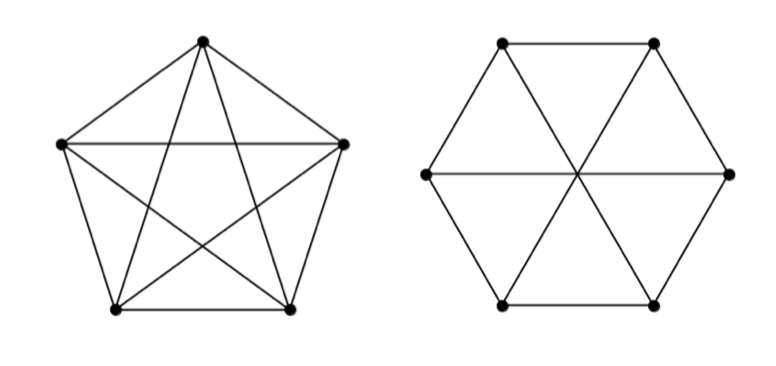
\includegraphics[width=.5\textwidth]{assets/images/Abb1-15-12-assignment.png}
    \end{figure}
  \end{enumerate} 
\end{assignment}
\begin{solution}
  \
  \begin{enumerate}[label= (\alph*)] 
    \item Sei \( n \geq 3 \), sei G ein planarer Graph mit \( k(G) \geq n \), so dass alle Kreise in G min. Länge \( n \) haben. \\
    \textbf{Zu zeigen:} \( k(G) \leq \frac{n}{n-2}(e(G) - 2) \). \\
    Sei oBdA \( G \) eben. Sei \( K \) die Menge der Kanten von \( G \), sei \( S \) die Menge der Flächenstücke von \( G \). \\
    Sei \( W = \{ (k,s) \in K \times S : k \text{ liegt auf dem Rand von S } \} \). \\
    Für alle \( k \in K \) gibt es höchstens zwei \( s \in S \) mit \( (k,s) \in W \), damit gilt \( \vert W \vert \leq 2 \vert K \vert \). \\
    Für alle \( s \in S \) gibt es mindestens \( n \) Kanten \( k \in K \), sodass \( (k,s) \in W \), denn falls \( s \) beschränkt ist, besteht der äußere Rand von \( s \) aus einem Kreis, der mindestens \( n \) Kanten hat (\emph{Vor.}). Wenn \( s \) unbeschränkt:
    \begin{itemize}
      \item \textbf{Fall 1}: \( G \) ist Baum. Dann ist \( s \) das einzige Flächenstück und alle Kanten berühren \( s \). (\( k(G) \geq n \)).
      \item \textbf{Fall 2}: \( G \) ist kein Baum, dann schließt \( s \) andere Flächenstücke ein, der Rand dieser Einschlüsse besteht aus einem oder mehreren Kreisen. Alle \( \geq n \) kanten dieser Kreise berühren \( s \).
    \end{itemize} 
    Also erhalten wir \( \vert W \vert \geq n \vert S \vert \). Wir erhalten \( n \cdot s(G) = n\vert S \vert \leq \vert W \vert \leq 2 \vert k \vert = 2k(G) \). \\
    Nach Eulerformel gilt: \\
    \( s(G) = k(G) - e(G) + 2 \), also \( \frac{2}{n}k(G) \geq \frac{n}{n} s(G) = k(G) - e(G) + 2 \).
    \begin{align*}
      &\Rightarrow \frac{2-n}{n}k(G) \geq - e(G) + 2 \\
      &\Rightarrow \frac{n-2}{n}k(G) \leq e(G) - 2 \\
      &\Rightarrow k(G) \leq \frac{n}{n-2}(e(G) - 2)
    \end{align*}
    \item Vgl. Zeichnungen:
    \begin{figure}[H]
      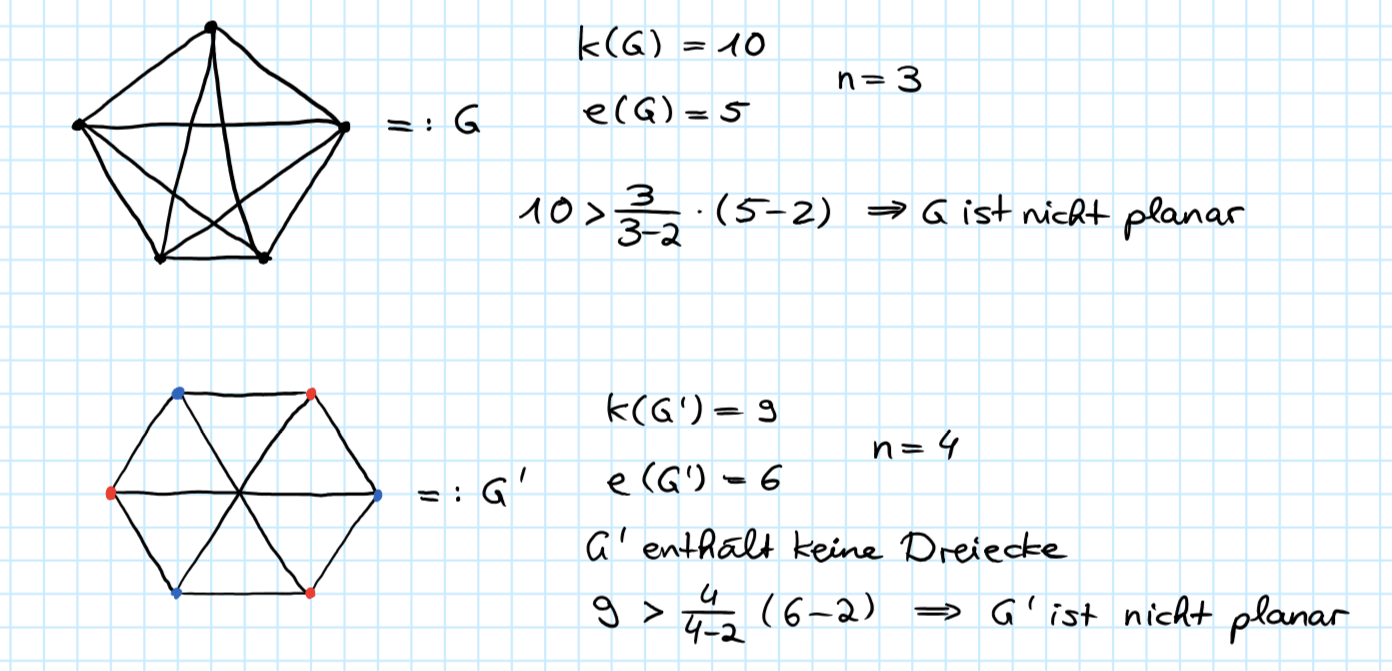
\includegraphics[width=\linewidth]{assets/images/Abb1-15-12.png}
    \end{figure}
  \end{enumerate} 
\end{solution}

\begin{assignment} 
  Für einen platonischen Körper \( P \subseteq \mathbb{R}^3 \) mit Zentrum \( 0 \) heißt die Gruppe
  \begin{align*}
    \text{Sym}(P) &\coloneqq \{ f \in O(3): f(P) = P \} 
  \end{align*} 
  \emph{Symmetriegruppe von P, und die Gruppe}
  \begin{align*}
    \text{Sym}_0(P) &\coloneqq \{ f \in SO(3): f(P) = P \}
  \end{align*}
  heißt \emph{eigentliche Symmetriegruppe von P}.
  
  Zeigen Sie für den Fall, dass \( P \) ein Würfel ist, folgende Aussagen: \\
  \begin{enumerate}[label= (\alph*)] 
    \item \( \text{Sym}(P) = S_4 \times \{ 1, -1 \} \) 
    \item \( \text{Sym}_0(P) = S_4 \) 
  \end{enumerate}
\end{assignment}
\begin{solution}
  \
  \begin{enumerate}[label= (\alph*)] 
    \item \textbf{Behauptung:} \\
    \( \vert \text{Sym}(P) \vert \leq 48, \vert \text{Sym}_0(P) \vert \leq 24 \). \\
    \textbf{Beweis:} Sei \( S \) eine Ecke von \( P \) und seien \( F,G,H \) die zu \( E \) benachbarten Ecken. Da \( \phi \) Ecken von \( P \) auf Ecken von \( P \) abbilden, gibt es nur 8 mögliche Werte von \( \phi(E) \). Da \( \phi \) benachbarte Ecken auf benachbarte Ecken von \( P \) abbildet, sind \( \phi(G), \phi(H), \phi(F) \) in einer von 6 Reihenfolgen die Nachbarn von \( \phi(E) \). Jetzt ist aber \( \phi \) vollständig durch \( \phi|_{\{ E,F,G,H \}} \) bestimmt, da \( E,F,G,H \) ein Erzeugendensystem von \( \mathbb{R}^3 \) ist. \\
    Damit ist \( \vert \text{Sym}(P) \vert \leq 6 \cdot 8 = 48 \). \\
    \( \text{Sym}_0(P) \) ist Untergruppe von \( \text{Sym}(P) \). \\
    Nach dem Satz von Lagrange ist \( \frac{\vert \text{Sym}(P) \vert}{\vert \text{Sym}_0(P) \vert} \in \mathbb{N} (\star) \). \\
    Da \( \begin{pmatrix}
      -1 & 0 & 0 \\
      0 & -1 & 0 \\
      0 & 0 & -1 
    \end{pmatrix} \in \text{Sym}(P) \), aber \( \det(-I) = {(-1)}^3 = -1 \),\\
    ist \( I \in \text{Sym}(P) \setminus \text{Sym}_0(P) \), also ist \( \vert \text{Sym}(P) \vert > \vert \text{Sym}_0(P) \vert \). \\
    Wegen \( (\star) \) folgt
    \begin{equation*}
      \frac{\vert \text{Sym}(P) \vert}{\vert \text{Sym}_0(P) \vert} \geq 2 \Rightarrow \vert \text{Sym}_0(P) \vert \leq \frac{1}{2} \vert \text{Sym}(P) \vert \leq 24.
    \end{equation*}
    Sei \( D \) die Menge der Hauptdiagonalen von \( P \). Dann ist 
    \begin{equation*}
      h: \text{Sym}_0(P) \to B_{ij}(D) \cong S_4, h(\phi) \coloneqq (d \mapsto \phi(d))
    \end{equation*}
    Gruppenhomomorphismus. \\
    
    \textbf{Behauptung:} \( h \) ist surjektiv. \\
    Da \( B_{ij}(D) \) von Transpositionen erzeugt wird reicht es zu zeigen, dass \( \text{Bild}(h) \) jede Transposition enthält. Sei also \( (d_1,d_2) \) eine beliebige Transposition in \( B_{ij}(D) \). \\
    Gesucht: \( \phi \in \text{Sym}_0(P) \) mit \( h(\phi) = (d_1,d_2). \) \\
    Wähle \( \phi \) als Rotation um \( 180^{\circ} \) um die gestrichelte Achse (vgl. Abb.), dann ist \( \phi(P) = P \), \( \det(\phi) = 1, \phi(RL) = BL, \phi(BL) = RL, \phi(GL) = GL, \phi(YL) = YL \). Wobei \( GL = \) Grüne Linie, etc. \\ 
    Damit ist \( h(\phi) = (d_1, d_2). \) \\
    Wir haben einen surjektiven Homomorphismus \( h: \text{Sym}_0(P) \to \underset{ \text{Bijektion}}{B_{ij}(D)} \). Aus \( \vert \text{Sym}_0(P) \vert \leq 24 = \vert S_4 \vert = \vert B_{ij}(D) \vert \) folgt sofort, dass \( \vert \text{Sym}_0(P) \vert = \vert B_{ij}(D) \vert \) ist und dass \( h \) bijektiv ist:
    \begin{equation*}
      \text{Sym}_0(P) \cong B_{ij}(D) \cong S_4.
    \end{equation*}
    \textbf{Behauptung:} \( \text{Sym}(P) \cong \text{Sym}_0(P) \times \{ -1, 1 \}. \) \\
    \textbf{Beweis:} Seien:
    \begin{align*}
      &g: \text{Sym}(P) \to \text{Sym}_0(P) \times \{ -1, 1 \}, \psi \mapsto (\det(\psi) \cdot \psi,\det(\psi)) \\
      &k: \text{Sym}_0(P) \times \{ -1, 1 \} \to \text{Sym}(P), (\phi, \varepsilon) \mapsto \varepsilon \phi.
    \end{align*}
    \textbf{Behauptung:} \( k,g \) sind zueinander Invers. \\
    \textbf{Bew:} 
    \begin{align*}
      g(k(\phi,\varepsilon)) &= g(\varepsilon \phi) = (\varepsilon^3 \cdot \varepsilon \phi, \varepsilon) = (\phi, \varepsilon) 
      \\
      k(g(\psi)) &= k(\det(\psi) \cdot \psi, \det(\psi)) = \det{(\psi)}^2 \cdot \psi = \psi
    \end{align*}
    \textbf{Behauptung:} \( k \) ist Hom. \\
    \textbf{Beweis:} 
    \begin{equation*}
      k((\phi, \varepsilon)\cdot (\phi', \varepsilon')) = k(\phi, \varepsilon) \cdot k(\phi',\varepsilon').
    \end{equation*}
    Damit folgt Behauptung. Also ist 
    \begin{equation*}
      \text{Sym}(P) \cong \text{Sym}_0(P) \times \{ -1, 1 \} \cong S_4 \times \{ -1, 1 \}.
    \end{equation*}
  \end{enumerate} 
\end{solution}

% ---------------------------------------------------------------------------------------
%
%----------------------------------------------------------------------------------------
\section{Übungsblatt 9}
\setcounter{problemcounter}{0}

\textbf{Definition zu Aufgabe 1 (Vgl. Blatt):} Eine triangulierte Fläche \( (M, K, t) \) besteht aus einer Fläche \( M \), einem Simplizialkomplex \( K \) und einem Homöomorphismus \( t: \vert K \vert \to M \). \\
\( (K, t) \) heißt \emph{Triangulierung} von \( M \). \\
Die Eulercharakteristik \( \chi(M) \) ist definiert als \( \chi(K) \), \( \chi(M) \) hängt also nicht von \( (K,t) \) ab.

\begin{assignment}
  Beschreibt diese Zeichnung eine Triangulierung des Torus \( T^2 \)?
  \begin{figure}[H]
    \centering
    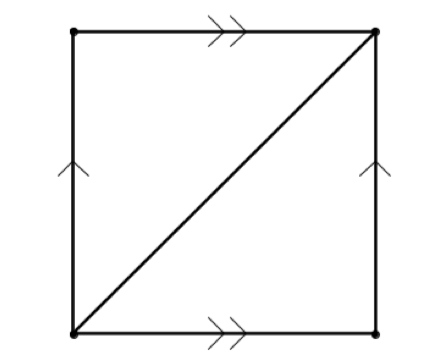
\includegraphics[width=.3\textwidth]{assets/images/triangulation_torus.png}
  \end{figure}
\end{assignment}

\begin{solution}
  \
  % TODO Zeichnung vom Übungsblatt
  \textbf{Antwort:} Nein! \\
  \textbf{Begründung:} In der Zeichnung werden alle Ecken identifiziert, aber Dreiecke in Simplizialkomplexen haben drei verschiedene Ecken (0-Simplices). Außerdem ist der Schnitt der zwei Dreiecke in er Zeichnung kein Simplex. \\
  \\
  \textbf{Überlegung:} Was ist dann eine korrekte Triangulierung des Torus \( T \)? \\
  
  % TODO Zeichnung einer korrekten Triangulierung mit 32 Dreiecken (4x4 kleine Quadrate)
  \textbf{Bonusfrage:} Wieviele Dreiecke braucht man mindestens, um einen Torus korrekt zu triangulieren? \\
  \textbf{Antwort:} 14! \\
  Sei \( (K,t) \) eine Triangulierung des Torus, sei 
  \begin{itemize}
    \item \( e \) die Anzahl der Ecken von \( K \).
    \item \( k \) die Anzahl der Kanten von \( K \).
    \item \( s \) die Anzahl der Dreiecke von \( K \).
  \end{itemize} 
  Zeichne auf jede Seite von jedem Dreieck ``innen'' einen Punkt. Sei \( x \) die Anzahl der Punkte.
  Da in jedem Dreieck drei Punkte liegen gilt \( x = 3s \). \\
  Da in jeder Kante zwei Punkte liegen gilt \( x = 2k \), also \( 3s = 2k \). \\
  Der Torus hat Euler-Charakteristik \( 0 \), also gilt
  \begin{equation*}
    3 \cdot 0 = 3 \cdot (s - k + e) = 3s - 3k +3e = \underbrace{(3s -2k)}_{= 0} - k + 3e \Rightarrow k = 3e
  \end{equation*}
  Damit ist \( 2e = \frac{2}{3} k = \frac{2}{3} s = s \). \\
  
  Da es \( \binom{e}{2} \) Paare von Ecken gibt und jede Kante ein anderes Eckenpaar als Enden hat, gilt \( \binom{e}{2} \geq k = 3e \). Da \( \binom{e}{2} \geq 3e \) erst ab \( e \geq 7 \) erfüllt ist, gilt \( e \geq 7 \), also \( s = 2e \geq 14 \). \\
  Um zu beweisen, dass der kleinste Wert für \( s \) genau \( 14 \) ist, reicht ein Beispiel: 
  
  % TODO Zeichnung mit 14 Dreiecken (vgl. Triangulation von Torus) 
\end{solution}

\begin{assignment}
  Seien \( M_1, M_2 \) zwei Flächen. Beweisen Sie die Gleichheit 
  \begin{equation*}
    \chi(M_1 \# M_2) = \chi(M_1) + \chi(M_2) - 2
  \end{equation*}
  Sie dürfen ohne Beweis verwenden, dass \( M_1 \# M_2 \) bis auf Homöomorphismus unabhängig von der Wahl der ausgeschnittenen Bälle und der Randverklebung ist, d.h.\ dass je zwei Mannigfaltigkeiten, die beide zusammenhängende Summen von \( M_1 \) und \( M_2 \) sind, zueinander homöomorph sind.
\end{assignment}
\begin{solution}
  \
  \textbf{Lemma 1}: Homöomorphe Flächen haben die gleiche Euler-Charakteristik. \\
  \textbf{Beweis}: Sei \( \phi : M \to \tilde{M} \) Homöomorphismus. Sei \( (K,t) \) eine Triangulierung von M. \\
  Dann ist \( (K,\phi \circ t) \) Triangulierung von \( \tilde{M} \), denn \( \phi \circ t \) ist Verkettung von Homöomorphismen. \\
  \  \\
  \textbf{Lemma 2}: Seien \( M_1, M_2, N_1, N_2 \) Flächen, sodass \( M_1 \cong N_1, M_2 \cong N_2 \). \\
  Dann ist \( M_1 \# M_2 \cong N_1 \# N_2 \). \\
  \textbf{Beweisansatz:} Seien \( \phi_1: M_1 \to N_1, \phi_2: M_2 \to N_2 \) Homöomorphismen. \\
  Sei \( M \coloneqq M_1 \# M_2 , N \coloneqq N_1 \# N_2 \) beliebige zusammenhängende Summen. \\
  Seien \( B_1 \subseteq M_1, B_2 \subseteq M_2 \) die Kreisscheiben, die zur Konstruktion von \( M \) verwendet wurden und sei \( F: \partial B_1 \to \partial B_2 \) der verwendete Homöomorphismus. \\
  Seien \( C_1 \coloneqq \phi_1 (B_1), C_2 \coloneqq \phi_2 (B_2) \). \\
  Sei dann \( \tilde{f} : \partial C_1 \to \partial C_2 \) gegeben durch 
  \begin{equation*}
    \tilde{f}(p) \coloneqq \phi_2 (f(\phi_1^{-1}(p)))
  \end{equation*}
  Sei \( \tilde{N} \) zusammenhängende Summe von \( N_1, N_2 \) mittels \( C_1, C_2, \tilde{f} \). \\
  Dann ist
  \begin{equation*}
    \phi: M \to \tilde{N}, [p] \mapsto \begin{cases}
      [\phi_1(p)]\text{,} &\text{falls } p \in M_1 \\
      [\phi_2(p)]\text{,} &\text{falls } p \in M_2
    \end{cases}
  \end{equation*}
  ein wohldefinierter Homöomorphismus. \\
  Also ist \( M \cong \tilde{N} \cong N \). \\
  
  \textbf{Beweis der Aufgabe:} \\
  Seien \( (K_1, t_1) \) und \( (K_2, t_2) \) Triangulierungen von \( M_1 \) und \( M_2 \). \\
  Jetzt ist nach \emph{Vorraussetzung} \( M_1 \cong \vert K_1 \vert, M_2 \cong \vert K_2 \vert \), also ist
  \begin{equation*} 
    M_1 \# M_2 \underset{ \text{ Lemma 2}}{ \cong} \vert K_1 \vert \# \vert K_2 \vert
  \end{equation*} 
  also auch: \( \chi (M_1 \# M_2) \underset{ \text{ Lemma 1}}{ =} (\vert K_1 \vert \# \vert K_2 \vert) \), wobei wir uns die Verklebung von \( \vert K_1 \vert \) und \( \vert K_2 \vert \) beliebig aussuchen dürfen. \\
  Seien also \( \triangle_1, \triangle_2 \) Dreiecke in \( K_1 \) bzw. \( K_2 \). \\
  Sei \( f: \partial \triangle_1 \to \partial \triangle_2 \) ein Homöomorphismus, der Ecken von \( \triangle_1 \) auf Ecken von \( \triangle_2 \) abbildet. \\
  Sei \( S \) die zusammenhängende Summe von \( \vert K_1 \vert \) und \( \vert K_2 \vert \) bzgl. 
  \( \triangle_1, \triangle_2, f \). \\
  Dann hat \( S \) eine durch \( K_1 \) und \( K_2 \) erzeugte simpliziale Struktur. \\
  Es gilt:
  \begin{align*}
    s(K) &= s(K_1) + s(K_2) - 2 \text{ da die Dreiecke fehlen} \\
    k(K) &= k(K_1) + k(K_2) - 3 \text{ da drei Kantenpaare verklebt wurden} \\
    e(K) &= e(K_1) + e(K_2) - 3 \text{ da drei Eckenpaare verklebt wurden}
  \end{align*}
  Also ist \( \chi(K) = \chi(K_1) + \chi(K_2) - 3 + 3 -2 = \chi(K_1) + \chi(K_2) - 2 \).
  Damit ist 
  \begin{align*}
    \chi(M_1 \# M_2) &= \chi(\vert K_1 \vert \# \vert K_2 \vert) \\
    &= \chi(S) = \chi(K) \\
    &= \chi(K_1) + \chi(K_2) - 2 \\
    &= \chi(M_1) + \chi(M_2) - 2.
  \end{align*} 
\end{solution}

\begin{assignment}
  Sei \( I \) ein Intervall und \( c: I \to \mathbb{R}^3 \) eine differenzierbare Kurve mit \( \frac{dc}{fs}(t) \neq 0 \) für alle \( t \in I \). \\
  Beweisen Sie, dass es ein Intervall J und ein Diffeomorphismus \( \varphi : I \to J \) gibt sodass für die umparametrisierte Kurve \( \tilde{c}: c \circ \phi^{-1} \) die Gleichung 
  \begin{equation*}
    \Vert \frac{d\tilde{c}}{ds}(s) = 1 \Vert
  \end{equation*}
  für alle \( s \in J \) erfüllt ist
\end{assignment}
\begin{solution}
  \
  \textbf{Beweis:} Sei \( a \in I \) beliebig. Sei \( \phi: I \to \mathbb{R} \) gegeben durch 
  \begin{equation*}
    \phi(x) \coloneqq \int_a^x { \Vert \frac{dc}{dt}(t) \Vert}dt
  \end{equation*}
  Da \( \Vert \frac{dc}{dt}(t) \Vert > 0 \) für alle \( t \in I \) ist, ist \( \phi \) stetig und streng monoton steigend, also ist \( \phi \) Homöomorphismus von \( I \) nach \( J \coloneqq \phi (I) \). \\
  Nach Konstruktion ist \( \phi \) stetig differenzierbar, woraus folgt:
  \begin{equation*}
    \left(\frac{d \phi}{dx}(x) = \Vert \frac{dc}{dt}(x) \Vert\right)
  \end{equation*}
  mit nicht verschwindender Ableitung, also ist \( \phi^{-1} \) auch überall stetig differenzierbar und damit ist \( \phi \) ein Diffeomorphismus. \\
  Sei nun \( \tilde{c} = c \circ \phi^{-1} \), sei \( s_0 \in J \) beliebig. Sei \( t_0 = \phi^{-1}(s_0) \). \\
  Jetzt gilt \( c = \tilde{c} \circ \phi \), mit Kettenregel folgt:
  \begin{align*}
    \frac{dc}{dt}(t_0) &= \frac{d \tilde{c}}{ds}(\phi(t_0))\cdot \frac{d \phi}{dt}(t_0) \\
    &\Rightarrow \Vert \frac{dc}{dt}(t_0)\Vert = \Vert \frac{d \tilde{c}}{ds}(s_0) \Vert \cdot \vert \frac{d \phi}{dt}(t_0) \vert = \Vert \frac{d \tilde{c}}{ds}(s_0) \Vert \cdot \Vert \frac{dc}{dt}(t_0) \Vert
  \end{align*}
  Kürzen mit \( \Vert \frac{dc}{dt} (t_0) \Vert \) ergibt \( 1 = \Vert \frac{d \tilde{c}}{ds}(s_0) \Vert \) wie gewünscht. \\
\end{solution}

% ---------------------------------------------------------------------------------------
%
%----------------------------------------------------------------------------------------
\section{Übungsblatt 10}
\setcounter{problemcounter}{0}

\begin{assignment}
  Sei \( U \coloneqq (0,1) \times (0, \infty) \). Gegen seien die parametrisierten Flächenstücke
  \begin{equation*}
    x : U \to \mathbb{R}^3, (u,v) \mapsto (\cos u, \sin u, v)
  \end{equation*} 
  und 
  \begin{equation*}
    x' : U \to \mathbb{R}^3, (u,v) \mapsto (u,v,0).
  \end{equation*}
  Geben Sie eine explizite lokale Isometrie von \( x(U) \) nach \( x'(U) \) an.
\end{assignment}
\begin{solution}
  \
  \textbf{Vorraussetzugen:} Vergleich Aufgabenstellung. \\
  \textbf{Beweis:} \\
  \emph{Erinnerung:} Sind \( x, x': U \to \mathbb{R}^3 \) Parametrisierte Flächenstücke und ist \( I_x(u,v) = I_{x'}(u,v) \) für alle \( (u,v) \in U \), dann sind \( x(U), x'(U) \) lokal isometrisch durch \( x' \circ x^{-1} \). \\
  \emph{Anwendung:} Berechne: \\
  \begin{align*}
    x_u = \begin{pmatrix} 
      -\sin(u) \\ \cos(u) \\ 0 
    \end{pmatrix},\enspace
    x_v = \begin{pmatrix} 
      0 \\ 0 \\ 1 
    \end{pmatrix},\enspace
    {x'}_u = \begin{pmatrix} 
      1 \\ 0 \\ 0 
    \end{pmatrix},\enspace
    {x'}_v= \begin{pmatrix} 
      0 \\ 1 \\ 0 
    \end{pmatrix}
  \end{align*}
  also gilt:
  \begin{equation*}
    I_x(u,v) = \begin{pmatrix}
      1 & 0 \\
      0 & 1
    \end{pmatrix}, \enspace
    I_x'(u,v) = \begin{pmatrix}
      1 & 0 \\
      0 & 1
    \end{pmatrix}
  \end{equation*}
  Also ist \( x' \circ x^{-1}: x(U) \to x'(U) \) die gesuchte lokale Isometrie. \\
  \emph{Optional:} Berechne explizite Darstellung von \( x' \circ x^{-1} \) 
  
\end{solution}

\begin{assignment}
  Eine \emph{Rotationsfläche} ist gegeben durch eine lokale Parametrisierung der Form
  \begin{align*}
    x:(0,2\pi) \times (a,b) &\to \mathbb{R}^3, \\
    (u,v) &\mapsto (\phi(v)\cos u, \phi(v)\sin u, \psi(v))
  \end{align*}
  Sie entsteht also durch die Rotation der Kurve \( v \mapsto (\phi(v), 0, \psi(v)) \) um die \( x_3 \)-Achse. \\
  Dabei gilt \( \phi, \psi: [a,b] \to \mathbb{R}, \phi \neq 0 \) und \( \frac{d}{dv}(\varphi(v), 0, \psi(v)) \neq (0,0,0) \) für alle \( v \in (a,b) \)
  \begin{enumerate}[label= (\alph*)] 
    \item Berechnen Sie die Gauß-Krümmung von x in Abhängigkeit von \( \varphi \) und \( \psi \). 
    \item Geben Sie Beispiele von Rotationsflächen mit konstanten Gauß-Krümmungen \( 0 \), \( 1 \) und \( -1 \) an.
  \end{enumerate}
\end{assignment}
\begin{solution}
  \
  \begin{enumerate}[label= (\alph*)] 
    \item Gegeben sei eine Rotationsfläche durch:
    \begin{align*}
      x:(0,2\pi) \times (a,b) &\to \mathbb{R}^3, \\
      (u,v) &\mapsto (\phi(v)\cos u, \phi(v)\sin u, \psi(v))
    \end{align*}
    
    \begin{equation*}
      x_u = \begin{pmatrix}
        -\phi(v)\sin(u) \\ \phi(v)\cos(u) \\ 0 
      \end{pmatrix}, \enspace
      x_v = \begin{pmatrix}
        -\phi'(v)\sin(u) \\ \phi'(v)\cos(u) \\ \psi'(v) 
      \end{pmatrix} 
    \end{equation*}
    Damit folgt: 
    \begin{align*}
      I_x(u,v) &= 
      \begin{pmatrix}
        {\phi(v)}^2 & 0 \\
        0 & {\phi'(v)}^2 + {\psi'(v)}^2 \\
      \end{pmatrix}, \\
      x_u \land x_v &= 
      \begin{pmatrix}
        \phi(v) \psi'(v) \cos u \\
        \phi(v) \psi'(v) \sin u \\
        -\phi(v) \phi'(v)
      \end{pmatrix}, \\
      \Vert x_u \land x_v \Vert &= \sqrt{ {\phi(v)}^2 {\psi'(v)}^2 + {\phi(v)}^2 {\phi'(v)}^2} \\
      &= \phi(v) \sqrt{ {\phi'(v)}^2 + {\psi(v)}^2}
    \end{align*}
    Damit folgt für \( n \):
    \begin{equation*}
      \centering
      n = \frac{1}{\sqrt{ {\phi'(v)}^2 + {\psi'(v)}^2}} \begin{pmatrix}
        \psi'(v) \cos(u) \\
        \psi'(v) \sin(u) \\
        -\phi(v)
      \end{pmatrix}
    \end{equation*}
    Weiter sind:
    \begin{align*}
      x_{uu} &= \begin{pmatrix}
        -\phi(v)\cos(u) \\
        -\phi(v) \sin u \\
        0
      \end{pmatrix}, \\
      x_{uv} &= \begin{pmatrix}
        -\phi(v)\sin(u) \\
        \phi(v) \cos u \\
        0
      \end{pmatrix} \\
      x_{vv} &= \begin{pmatrix}
        -\phi''(v)\cos(u) \\
        \phi''(v) \sin u \\
        \psi''(v)
      \end{pmatrix} 
    \end{align*}
    Damit ist dann: 
    \begin{align*}
      \rom{2}_x(u,v) &= \frac{1}{\sqrt{ {\phi'(v)}^2 + {\psi'(v)}^2}} \cdot \begin{pmatrix}
        -\phi(v) \psi(v) & 0 \\
        0 & \phi''(u) \psi'(v) - \psi'(u)\psi'(v)
      \end{pmatrix} \\ 
      K &= \frac{\det(\rom{2})}{\det(\rom{1})} = \phi \cdot \psi'
    \end{align*}
    \emph{Anmerkung:} Hier bin ich mir mit den Variablen von \( \phi, \psi \) nicht ganz sicher. Für Verbesserungen gerne melden.
    
    \item 
    Wir suchen für ein vorgegebenes \( K \) solche \( \phi, \psi \) sodass (\*) erfüllt wird. Um unsere Suche einzuschränken, können wir Bedingungen an \( \phi, \psi \) stellen. \\
    \emph{Beispiel}: Fordern wir, dass \( \psi(v) = v \) gilt. Aus (*) folgt dann 
    \begin{equation*}
      K = \frac{-\phi''}{\phi{(\phi'^2 + 1)}^2}
    \end{equation*} 
    das heißt:
    \begin{equation*}
      \phi'' = -K \phi \cdot {(\phi'^2 + 1)}^2
    \end{equation*} 
    \emph{\textbf{Zitat:}} \emph{``Das ist nicht so schön, es ist sogar ziemlich hässlich.''} \\
    Es zeigt uns aber, dass Lösungen existieren. \\
    Versuchen wir eine andere Bedingungen an \( \phi, \psi \) zu stellen. \\
    Wir können fordern, dass die Kurve \( v \mapsto (\phi(v), 0, \psi(v)) \) nach Bogenlänge parametrisiert ist. Das heißt, dass \( \phi'^2 + \psi'^2 = 1 \). (+)\\
    Also gilt auch:
    \begin{equation*}
      0 = \frac{d}{dv}(\phi'^2 + \psi'^2) = 2 \phi'\phi'' + 2 \psi' \psi''
    \end{equation*}
    Nun ist 
    \begin{equation*}
      K = \frac{\phi' \psi' \psi'' - \psi'^2 \phi''}{\phi\underbrace{{(\phi'^2 + \psi'^2)}^2}_{= 1}} = \frac{-\phi'^2 \phi'' - \psi'^2 \phi''}{\phi} = \frac{-\phi''}{\phi}
    \end{equation*}
    Damit ist \( \phi'' = -K \phi \) (**) \\
    \textbf{Fall K = 1}: \\
    Die Lösungen von \( \phi'' = - \phi \) sind \( \phi(v) = a \cos v + b \sin v (a,b \in \mathbb{R}) \). \\
    Suchen wir uns \( \phi(v) = \cos v \) aus, so können wir \( \phi(v) = \sin v \) wählen, um (+) zu erfüllen. \\
    Dann ist
    \begin{equation*}
      x(u,v) = \begin{pmatrix}
        \cos(v) \cos(u) \\
        \cos(v) \sin(u) \\
        \sin(v) 
      \end{pmatrix}
    \end{equation*}
    und das ist genau die Parametrisierung der 2-Sphäre. \\
    \textbf{Fall K = 0:} \\
    Aus (**) folgt \( \phi'' = 0 \) das heißt: \\
    \( \phi(v) = av + b, \psi(v) = cv + d \) mit \( \sqrt{ a^2 + c^2} = 1 \), damit (+) gilt. \\
    
    % TODO: Schaubild für Kegelausschnitt oder Fläche mit K = 0
    
    \textbf{Fall K = -1:} Aus (**) folgt dann \( \phi'' = \phi \), das heißt: \\
    \( \phi(v) = a \cdot e^v + b \cdot e^{-v} (a,b \in \mathbb{R}) \)  \\
    Wir suchen uns \( \phi(v) = e^v \) aus, dann ist wegen (+)
    \begin{equation*}
      \psi'(v) = \sqrt{ 1- e^{2v}}, \text{ und} \psi(v) = \int{ \sqrt{ 1 - e^{2v}}}dv = \sqrt{ 1 - e^{2v}} -\tanh^{-1}(\sqrt{ 1- e^{2v}}).
    \end{equation*}
    \emph{\textbf{Zitat:}} \emph{``Wie man darauf kommt, weiß ich auch nicht.''}
    
    % TODO: Schaubild für halbe Pseudosphäre mit K = -1
  \end{enumerate} 
\end{solution}

\begin{assignment}
  Sei \( S \) eine reguläre Fläche und \( c: (0,l) \to S, t \mapsto c(t) \) eine nach Bogenlänge parametrisierte Flächenkurve. \\
  Weiter sei \( \tilde{ c } : (0,l) \to S \) die Umparametrisierung von \( c \) gegeben durch \( \tilde{ c }(t) \coloneqq c(l-t) \). Zeigen Sie, dass für die geodätischen Krümmungen \( \kappa_g \) und \( \tilde{ \kappa }_g \) von \( c \) und \( \tilde{ c } \) gilt: 
  \begin{equation*}
    -\tilde{\kappa}_g(t) = k_g(l-t) 
  \end{equation*}
\end{assignment}
\begin{solution}
  \emph{Erinnerung:} Für eine nach Bogenlänge parametrisierte Flächenkurve c ist \( \{ c', n \land c', n \} \) eine ONB an jedem Punkt \( c(t) \). \\
  Es ist \( c''(t) = 0 \cdot c'(t) + \kappa_g(t)(n(t) \land c'(t)) + \alpha(t) n(t) \). \\
  Da die Normale \( n \) nicht von der Parametrisierung von \( c \) abhängt gilt \( \tilde{n}(t) = n(l-t) \). \\
  Weiter gilt \( \tilde{c}'(t) = \frac{d}{dt}[c(l-t)] = - c'(l-t) \) und \\
  \( \tilde{c}''(t) = \frac{d}{dt}[\tilde{c}'(t)] = c''(l-t) \) und \\
  \( \tilde{n}(t) \land \tilde{c}'(t) = n(l-t) \land - c'(l-t) = -n (l-t) \land c'(l-t) \). \\
  Also ist:
  \begin{align*}
    & 0c'(l-t) + \kappa_g(l-t)(n(l-t) \land c'(l-t)) + \alpha(l-t)n(l-t) = c''(l-t) \\
    &= \tilde{c}''(t) = 0\tilde{c}'(t) + \tilde{\kappa_g}(t)(\tilde{n}(t) \land \tilde{c}(l-t) + \tilde{\alpha}(t) \tilde{n}(t)) \\
    &= -0 c'(l-t) - \tilde{\kappa_g}(t)(n(l-t) \land c'(l-t)) + \tilde{\alpha}(t) \cdot n(l-t)
  \end{align*}
  Durch Koeffizientenvergleich: \\
  \( -0 = 0 \text{ und} \tilde{\alpha}(t) = \alpha(l-t) \). \\
  Daraus folgt direkt die Behauptung.
\end{solution}

% ---------------------------------------------------------------------------------------
%
%----------------------------------------------------------------------------------------
\section{Übungsblatt 11}
\setcounter{problemcounter}{0}

\begin{assignment}
  Seien \( R, r \in \mathbb{R} \) mit \( R > r > 0 \) und sei \( T^2(R,r) \) der Rotationstorus gegeben durch die lokale Parametrisierung der Form
  \begin{equation*}
    x: U \to \mathbb{R}^3, (u,v) \mapsto \begin{pmatrix}
      (R + r\cos u) \cos v \\
      (R + r\cos u) \sin v \\
      r \sin v
    \end{pmatrix}
  \end{equation*}
  wie in Aufgabe 4 von Übungsblatt 9. Bestimmen und skizzieren Sie die Bereiche von \( T^2(R,r) \) mit positiver, negativer und verschwindender Gauß-Krümmung 
\end{assignment}
\begin{solution}
  \
\end{solution}
\emph{Erster Weg:} Gauß-Krümmung ausrechnen und entsprechend auflösen. \\
\( \rightarrow \) Rechenaufwand! \\
\emph{Zweiter Weg:} In der letzten Übung haben wir die Gauß-Krümmung von Rotationsflächen bestimmt.
\begin{equation*}
  x(u,v) = \begin{pmatrix}
    \phi(u) \cos(v) \\
    \phi(u) \sin(v) \\
    \psi(u) 
  \end{pmatrix}
\end{equation*}
Dann ist die Gauß-Krümmung gegeben durch: 
\begin{equation*} 
  K(u,v) = \frac{\phi' \psi' \psi'' - \phi'' \psi'^2}{\phi(\phi'^2 + \psi'^2)}
\end{equation*}
Für \( \phi(u) = R + r \cos u, \psi(u) = r \sin u \) erhalten wir:
\begin{align*}
  K(u,v) &= \frac{-(r \sin u)(r \cos u)(-r \sin u)-(-r \cos u){(r \cos u)}^2}{(R+r \cos u)({(-r \sin u)}^2 + {(r \cos u)}^2)} \\
  &= \frac{r^3(\cos u(\sin^3u + \cos^3 u))}{ (R + r \cos u) r^4} \\
  &= \frac{\cos u}{r(R+r \cos u)} 
\end{align*}
Da weiter \( r(R + r \cos u) > 0 \) ist, folgt: 
\begin{align*}
  K > 0 &\Leftrightarrow \cos u > 0 \\
  K = 0 &\Leftrightarrow \cos u = 0 \\
  K < 0 &\Leftrightarrow \cos u < 0
\end{align*}
\begin{problem}[1]
  
  \begin{assignment}
    Eine Teilmenge \( U \subseteq \bar{\mathbb{C}} \) heißt offen in \( \bar{\mathbb{C}} \coloneqq \mathbb{C} \cup \left \{ \infty \right \} \), falls \( U \cap \mathbb{C} \) offen in der Standardtopologie von \( \mathbb{C} \cong \mathbb{R}^2 \) ist und falls im Falle \( \infty \in U \) das Komplement \( \mathbb{C} \setminus U \) beschränkt ist. Dies definiert eine Topologie auf \( \bar{\mathbb{C}} \).
    Zeigen Sie, dass \( \bar{\mathbb{C}} \) mit dieser Topologie kompakt ist.
  \end{assignment}
  \begin{solution}
    \
    \textbf{Beweis:} Sei \( \ddot{U} \) eine offene Überdeckung von \( \bar{\mathbb{C}} \). \\
    Wähle \( U_{\infty} \in U \), sodass \( \infty \in U_{\infty} \). Dann ist \( U_{\infty} \cap \mathbb{C} \) offen in \( \mathbb{C} \), also ist \( \bar{\mathbb{C}} \setminus U_{\infty} = \mathbb{C} \setminus U_{\infty} \) abgeschlossen und beschränkt. Nach Heine-Borel ist \( \bar{\mathbb{C}} \setminus U_{\infty} \) also kompakt. \\
    Die Menge \( U \coloneqq \{ \tilde{\ddot{U}} \setminus U_{\infty} : U \in \ddot{U} \} \) ist offene Überdeckung von \( \bar{\mathbb{C}} \setminus U_{\infty} \), denn für alle \( x \in \bar{\mathbb{C}} \setminus U_{\infty} \) gibt es ein \( U_x \in \ddot{U} \) mit \( x \in U_x \), also auch \( \tilde{\ddot{U}_x} \coloneqq U_x \setminus U_{\infty} \in \tilde{\ddot{U}} \) mit \( x \in \tilde{U_x}. \) \\
    Da \( \tilde{\ddot{U}} \) offene Überdeckung einer kompakten Menge ist hat \( \tilde{\ddot{U}} \) eine endliche Teilüberdeckung: 
    \begin{equation*}
      \{ U_1 \setminus U_{\infty}, \dots, U_n \setminus U_{\infty} \}, U_1, \dots, U_n \in \ddot{U}
    \end{equation*}
    Dann ist \( \{ U_1, \dots, U_n, U_{\infty} \} \) eine endliche Teilüberdeckung von \( \ddot{U} \), denn für alle
    \( x \in \bar{\mathbb{C}} \) ist entweder \( x \in U_{\infty} \), oder \( x \notin U_{\infty} \) aber im zweiten Fall gibt es \( i \in \{ 1, \dots, n \} \) mit 
    \begin{equation*}
      x \in U_i \setminus U_{\infty} \subseteq U_i
    \end{equation*} 
    also \( x \in U_i \). 
  \end{solution}
\end{problem}

\begin{assignment}
  Sei \( A = \begin{pmatrix}
    a & b \\
    c & d 
  \end{pmatrix} \in GL(2,\mathbb{C}) \) \\
  Die Abbildung
  \begin{equation*}
    M_A : \bar{\mathbb{C}} \to \bar{\mathbb{C}}, z \mapsto \frac{az + b}{cz + d}, \infty \mapsto \frac{a}{c}
  \end{equation*}
  heißt von \( A \) induzierte \emph{Möbiustransformation}. \\
  Zeigen Sie, dass \( M_A \) bijektiv ist.
\end{assignment}
\begin{solution}
  \
  \textbf{Voraussetzung}: Sei \( A = \begin{pmatrix}
    a & b \\
    c & d 
  \end{pmatrix} \in GL(2,\mathbb{C}) \) 
  \textbf{Zu zeigen}:
  
  bijektiv ist. \\
  \textbf{Beweis}: Benutzt folgendes Lemma: \\
  \textbf{Lemma}: Für alle \( A,B \in GL(2, \mathbb{C}) \) ist \( M_A \circ M_B = M_{A \cdot B} \). \\
  \emph{Beweis des Lemmas}: \\
  Sei \( A = \left(\begin{smallmatrix}
    a & b \\
    c & d
  \end{smallmatrix} \right), B = \left(\begin{smallmatrix}
    e & f \\
    g & h
  \end{smallmatrix} \right) \). \\
  
  % TODO: FIX smallmatrix
  
  \textbf{Fall 1}: \( Z \neq \infty, gz+h \neq 0 \). \\
  Dann ist:
  \begin{align*}
    M_A(M_B(z)) &= M_A\left(\frac{ez+f}{gz+h} \right) = \frac{a(\frac{ez+f}{gz+h}) + b}{c(\frac{ez+f}{gz+h}) + d} \\
    &= \frac{a(ez+f)+b(gz+h)}{c(ez+f)+d(gz+h)} = \frac{(ae+bg)z + (af+bh)}{(ce+dg)z + (cf +dh)} \\
    &= M_{\left(\begin{smallmatrix}
      ae+bg & af+bh \\
      ce+dg & cf+dh 
    \end{smallmatrix} \right)}
  \end{align*}
  \textbf{Fall 2}: \( gz+h = 0 \) \\
  \begin{align*}
    M_A(M_B(z)) &= M_A\left(\frac{ez+f}{gz+h} \right) = M_A(\infty) = \frac{a}{c} = \frac{a(ez+f)}{c(ez+f)} \\
    &= \frac{a(ez+f) + b(gz+h)}{c(ez+f)+d(gz+h)} \\
    &= M_{AB}(z)
  \end{align*}
  \textbf{Fall 3}: Für \( z = \infty, g \neq 0 \): 
  \begin{align*}
    M_A(M_B(\infty)) = M_A\left(\frac{e}{g} \right) = \frac{a \cdot \frac{e}{g} + b}{c \cdot \frac{e}{g} + d}
    = \frac{ae + bg}{ce+dg} = M_{AB}(\infty) 
  \end{align*}
  \textbf{Fall 4}: \( z = \infty, g = 0: \) 
  \begin{align*}
    M_A(M_B(\infty)) = M_A\left(\frac{e}{g} \right) = M_A(\infty) = \frac{a}{c} = \frac{ae}{ce} = \frac{ae + bg}{ce + dg} = M_{AB}(\infty) 
  \end{align*}
  \textbf{Beweis Aufgabe}: Sei nun \( A \in GL(2,\mathbb{C}) \) beliebig. Nach Lemma ist:
  \begin{equation*}
    M_A \circ M_{A^{-1}} = M_{\left(\begin{smallmatrix}
      1 & 0 \\
      0 & 1 
    \end{smallmatrix} \right)} = M_{A^{-1}} \circ M_A
  \end{equation*}
  und 
  \begin{equation*}
    M_{\begin{smallmatrix}
      1 & 0 \\
      0 & 1 
    \end{smallmatrix}} : z \mapsto \frac{1z+0}{0z+1} = z, \infty \mapsto \frac{1}{0} = \infty 
  \end{equation*}
  also ist \( M_A \) Umkehrfunktion zu \( M_A \), also ist \( M_A \) bijektiv. \\
\end{solution}


\begin{assignment}
  Sei \( D^2 \coloneqq \left \{ z \in \mathbb{C} : \vert z \vert < 1 \right \} \) die Einheitskreisscheibe in \( \mathbb{C} \) und \( H^2 \coloneqq \left \{ z \in \mathbb{C} : Im z > 0 \right \} \) die obere Halbebene in \( \mathbb{C} \). \\
  Bezüglich der Topologie auf \( \bar{\mathbb{C}} \) ist \( \bar{ D^2 } = \left \{ z \in \mathbb{C} : \vert z \vert \leq 1 \right \} \) und \( \tilde{H^2} \coloneqq \left \{ z \in \mathbb{C} : Im z \geq 0 \right \} \cup \left \{ \infty \right \} \). \\
  Sei nun
  \begin{equation*}
    M: \bar{\mathbb{C}} \to \bar{\mathbb{C}}, z \mapsto \frac{iz + 1}{z + c}, \infty \mapsto i
  \end{equation*}
  eine ausgewählte Möbiustransformation. Zeigen Sie
  \begin{enumerate}[label= (\alph*)] 
    \item \( M(H^2) = D^2 \)
    \item \( M(\bar{ H^2 }) = \bar{ D^2 } \)
    \item \( M(\mathbb{R} \cup \left \{ \infty \right \}) = S^1 \)
  \end{enumerate}
\end{assignment}
\begin{solution}
  \
  Seien \( A_1 \coloneqq \{ z \in \mathbb{C}: Im z > 0 \} = H^2 \), \\
  \( A_2 \coloneqq \{ z \in \mathbb{C}: Im z < 0 \} \),\\
  \( A_3 \coloneqq \{ z \in \mathbb{C}: Im z = 0 \} \cup \{ \infty \} = \bar{\mathbb{R}} \),\\
  \( B_1 \coloneqq \{ z \in \mathbb{C} : \vert z \vert < 1\} = D^2 \), \\
  \( B_2 \coloneqq \{ z \in \mathbb{C} : \vert z \vert > 1\} \cup \{ \infty \} \),\\
  \( B_3 \coloneqq \{ z \in \mathbb{C} : \vert z \vert = 1\} = S^1 \),\\
  \textbf{Behauptung:} \( M(A_i) = B_i \) für \( i = 1, 2, 3 \).
  
  \begin{itemize}
    \item[\( \subseteq \):] \emph{Bemerkung:} \( \bar{\mathbb{C}} = A_1 \cup A_2 \cup A_3 \). \\
    Sei \( z \in \bar{\mathbb{C}} \) beliebig. \\
    \begin{itemize}
      \item \textbf{Fall 1:} \( z = 0 \). Dann ist \( z \in A_3 \) und \( M(z) = i \in B_3 \).
      \item \textbf{Fall 2:} \( Z = -i \). Dann ist \( z \in A_2 \) und \( M(z) = \infty \in B_2 \).
      \item \textbf{Fall 3:} \( z = a+ib \in \mathbb{C}, z \neq -i \). Dann ist:
      \begin{equation*}
        M(z) = \frac{i(a+ib) + 1}{a + ib + i} = \frac{i (a+ib -i)}{a + ib + i}
      \end{equation*}
      also
      \begin{equation*}
        \vert M(z) \vert = \frac{\vert a+ib-i \vert}{a+ib-i} = \frac{\sqrt{ a^2 + {(b-1)}^2}}{\sqrt{ a^2 + {(b+1)}^2}}
      \end{equation*}
      Da gilt:
      \begin{align*}
        {(b+1)}^2 > {(b-1)}^2 \Leftrightarrow b > 0 \\
        {(b+1)}^2 = {(b-1)}^2 \Leftrightarrow b = 0 \\
        {(b+1)}^2 < {(b-1)}^2 \Leftrightarrow b < 0 \\
      \end{align*}
      gilt dasselbe auch für \( \vert M(z) \vert \).
      \begin{enumerate}
        \item \textbf{Fall 3.1}: \( b > 0 \Rightarrow z \in A_1, M(z) \in B_1 \) 
        \item \textbf{Fall 3.2}: \( b = 0 \Rightarrow z \in A_3, M(z) \in B_3 \) 
        \item \textbf{Fall 3.3}: \( b < 0 \Rightarrow z \in A_2, M(z) \in B_2 \) 
      \end{enumerate}
    \end{itemize}
    
    \item[\( \supseteq \):] \emph{Bemerkung:} \( \bar{\mathbb{C}} = B_1 \cup B_2 \cup B_3 \). \\
    \( M \) ist Möbiustransformation, also surjektiv. \\
    Angenommen, \( \exists z \in \bar{\mathbb{C}} \) mit \( z \in B_i \), aber \( z \notin M(A_1) \) für ein \( i \in \{ 1, 2, 3 \} \). \\
    oBdA \( i = 1 \) \\
    Für dieses \( z \) gilt:
    \begin{itemize}
      \item \( z \in M(A_1) \) nach Annahme,
      \item \( z \in B_2 \supseteq M(A_2) \) wegen \( B_1 \cap B_2 = \varnothing \),
      \item \( z \in B_3 \supseteq M(A_3) \) wegen \( B_1 \cap B_3 = \varnothing \),
    \end{itemize}
    Damit ist
    \begin{equation*}
      z \in M(A_1) \cup M(A_2) \cup M(A_3) = M(A_1 \cup A_2 \cup A_3) = M(\bar{\mathbb{C}}) = \bar{\mathbb{C}} \hfill \lightning
    \end{equation*}
    Damit ist dann:
    \begin{enumerate}[label= (\alph*)] 
      \item \( M(H^2) = M(A_1) = B_1 = D^2 \hfill \checkmark \) 
      \item \( M(\bar{H^2}) = M(A_1 \cup A_3) = M(A_1) \cup M(A_3) = B_1 \cup B_3 = \bar{D^2} \hfill \checkmark \) 
      \item \( M(\bar{ \mathbb{R}}) = M(A_3) = B_3 = S^1 \hfill \checkmark \) \\
    \end{enumerate}
  \end{itemize}
\end{solution}

% ---------------------------------------------------------------------------------------
%
%----------------------------------------------------------------------------------------
\section{Übungsblatt 12}
\setcounter{problemcounter}{0}

\begin{assignment}
  Zeigen Sie: Kreise und Geraden in \( \mathbb{C} \cong \mathbb{R}^2 \) sind genau diejenigen Teilmengen von \( \mathbb{C} \), die man in der Form
  \begin{equation*}
    \{ z \in \mathbb{C} : \alpha z \bar{z}+ \beta z + \bar{\beta} \bar{z} + \gamma = 0 \} 
  \end{equation*}
  schreiben kann, wobei \( \alpha, \gamma \in \mathbb{R}, \beta \in \mathbb{C}, \beta \cdot \bar{ \beta} > \alpha \gamma \).
\end{assignment}
\begin{solution}
  \
  \textbf{Beweis:}
  \begin{itemize}
    \item Sei \( K \) ein Kreis in \( \mathbb{C} \) mit Mittelpunkt \( w \in \mathbb{C} \), Radius \( r < 0 \):
    \begin{align*} 
      K &= \{ z \in \mathbb{C} : \vert z - w \vert = r \} \\
      &= \{ z \in \mathbb{C} : (z - w)(z-w) = r^2\} \\
      &= \{ z \in \mathbb{C} : z \bar{z} - w \bar{z} - \bar{z} w + w \bar{w} - r^2 = 0 \} \\
      &= \{ z \in \mathbb{C} : \alpha z \bar{z} + \beta z + \bar{\beta} \bar{z} + \gamma = 0 \} \\
      \alpha &= 1, \enspace \beta = - \bar{w}, \enspace \gamma = w \bar{w} - r^2
    \end{align*}
    Hier ist \( \beta \bar{\beta} = \bar{w}w > \bar{w} w - r^2 = \gamma = \alpha \gamma \).
    \item Sei \( L \) eine Gerade in \( \mathbb{C} \) mit Normale \( n \in S^1 \subset \mathbb{C} \) und \( x \in L \). Dann ist \( L - x \) eine Gerade mit Normale \( n \) durch \( 0 \) und \( \bar{n}(L -x) \) eine Gerade mit Normale \( 1 \) durch \( 0 \), also die imaginäre Achse.
    Also ist 
    \begin{align*}
      L &= \{ z \in \mathbb{C}: 2 Re(\bar{n}(z - x)) = 0 \} \\
      &= \{ z \in \mathbb{C}: \bar{n}(z-x) + (\bar{n}(z - x)) = 0 \} \\
      &= \{ z \in \mathbb{C}: \bar{n}z + n \bar{z} - \bar{n}x - n \bar{x}= 0 \} \\
      &= \{ z \in \mathbb{C}: \alpha z \bar{z} + \beta z + \bar{\beta} \bar{z} + \gamma = 0 \} \\
      \alpha &= 0, \enspace \beta = \bar{n}, \enspace \gamma = -n \bar{x} - \bar{n} x \\
      \beta \bar{\beta} &= \vert n \vert^2 = 1 > 0 = 0 \gamma = \alpha \gamma
    \end{align*} 
    \item \( M = \{ z \in \mathbb{C} : \alpha z \bar{z} + \beta z + \bar{\beta} \bar{z} + \gamma = 0 \}, \bar{\beta} \cdot \beta > 0 \) \\
    \textbf{Fall 1}: \( \alpha \neq 0 \). Dann ist
    \begin{align*}
      M &= \{ z \in \mathbb{C} : z \bar{z} + \frac{\beta}{\alpha}z + \frac{\bar{\beta}}{\alpha} \bar{z} + \frac{\beta \bar{\beta}}{\alpha^2} - \frac{\beta \bar{\beta}}{\alpha^2} + \frac{\gamma}{\alpha} = 0\} \\
      &= \{ z \in \mathbb{C} : (z + \frac{\bar{\beta}}{\alpha})(\bar{z} + \frac{\beta}{\alpha}) = \underbrace{\frac{\beta \bar{\beta}}{\alpha^2} - \frac{\alpha \gamma}{\alpha}}_{> 0} \} \\
      &= \{ z \in \mathbb{C} : \vert z + w \vert^2 = r^2\}
    \end{align*}
    Also ist \( M \) der Kreis um \( w = -\frac{\bar{\beta}}{\alpha} \) mit Radius \( r = \sqrt{ \frac{1}{\alpha} (\beta \bar{\beta} - \alpha \gamma)} \) \\
    \textbf{Fall 2}: \( \alpha = 0 \), also \( \beta \neq 0 \). \\
    \begin{align*}
      M &= \left \{ z \in \mathbb{C} : \frac{\beta}{\vert \beta \vert} z + \frac{\bar{\beta}}{\vert \beta \vert} \bar{z} + \frac{\gamma}{\vert \beta \vert} = 0 \right \} \\
      &= \left \{ z \in \mathbb{C} : \left(\frac{\beta}{\vert \beta \vert} + \frac{\gamma}{z\vert \beta \vert} \right) + \left(\frac{\beta}{\vert \beta \vert}z + \frac{\gamma}{z\vert \beta \vert} \right)= 0 \right \} \\
      &= \left \{ z \in \mathbb{C} : Re(\bar{n}(z-x)) = 0 \right \} \\
      &\text{ wobei} \\
      n &= \frac{\bar{\beta}}{\vert \beta \vert}, x = \frac{-n \gamma}{2\vert \beta \vert} 
    \end{align*}
    Dies ist eine Gerade mit Normale \( n \) durch \( x \).
  \end{itemize}
\end{solution}
\begin{assignment}
  Gegeben sei die Abbildung
  \begin{equation*}
    J: \bar{\mathbb{C}} \to \bar{\mathbb{C}}, z \mapsto \frac{-1}{z}, 0 \mapsto \infty, \infty \mapsto 0
  \end{equation*}
  \begin{enumerate}[label= (\alph*)] 
    \item Zeigen Sie: Für jeden Kreis und jede Gerade \( K \subseteq \bar{\mathbb{C}} \) ist \( J(K) \) ein Kreis oder eine Gerade in \( \bar{\mathbb{C}} \)
    \item Ist \( J\bigg\rvert_{ H^2 } \) eine Möbiustransformation?
  \end{enumerate}
\end{assignment}
\begin{solution}
  \
  \begin{enumerate}[label= (\alph*)] 
    \item \emph{Anmerkung:} Geraden in \( \bar{\mathbb{C}} \) enthalten \( \infty \). \\
    \emph{Bemerkung:} J ist selbstinverse Bijektion, also kann man Mengen der Form \( \{ J(Z): z \in \mathbb{C}, \text{ Eigenschaft} (z) \} \), auch so schreiben: \\
    \( \{ z \in \mathbb{C} : Eigenschaft J(z) \} \). \\
    Nach Aufgabe 1 kann man Kreislinien in \( \mathbb{C} \) so darstellen: \\
    \begin{align*}
      M_{\alpha, \beta, \gamma} &\coloneqq \{ z \in \mathbb{C} \setminus \{ o \} : \alpha z \bar{z} + \beta z + \bar{\beta} \bar{z} + \gamma = 0 \} \\
      &\cup \{ 0 : \gamma = 0 \} \cup \{ \infty : \alpha = 0 \}
    \end{align*}
    Nun ist:
    \begin{align*}
      J(M_{\alpha, \beta, \gamma}) &= \left \{ J(z): z \in \mathbb{C} \setminus \{ 0 \}, \alpha z \bar{z} + \beta z + \bar{\beta} \bar{z} \right \} \\
      &\cup \left \{ J(0): \gamma = 0 \right \} \\
      &\cup \left \{ J(\infty): \alpha = 0 \right \} \\
      &= \left \{ z \in \mathbb{C} \setminus \{ 0 \} : \alpha \cdot \frac{-1}{z} \cdot \frac{-1}{z} + \beta \cdot \frac{-1}{z} + \beta \cdot \frac{-1}{z} + \gamma = 0 \right \} \\
      &\cup \left \{ \infty : \gamma = 0 \right \} \\
      &\cup \left \{ 0 : \alpha = 0 \right \} \\
      &= \left \{ z \in \mathbb{C} \setminus \{ 0 \} : \alpha - \beta \bar{z} - \bar{\beta}z + \gamma z \bar{z} = 0 \right \} \\
      &\cup \left \{ 0 : \alpha = 0 \right \} \\
      &\cup \left \{ \infty : \gamma = 0 \right \} = M_{\tilde{\alpha}, \tilde{\beta} \tilde{\gamma}}
    \end{align*}
    mit
    \begin{align*}
      &\tilde{\alpha} = \gamma, \tilde{\gamma} = \alpha, \tilde{\beta} = - \bar{\beta}.
    \end{align*}
    Das ist eine Kreislinie.
    \item \textbf{Antwort:} Ja, denn \( J: z \mapsto \frac{-1}{z} = \frac{0z - 1}{1z + 0}, \infty \mapsto 0 = \frac{0}{1} \). \\
    Also ist \( J \) die Möbiustransformation zur Matrix
    \begin{equation*}
      M = \begin{pmatrix}
        0 & -1 \\
        1 & 0 
      \end{pmatrix} \in SL(2,\mathbb{R})
    \end{equation*}
    also eine \( H^2 \)- Möbiustransformation.
  \end{enumerate} 
\end{solution}

\begin{assignment}
  Sei \( L \) ein Halbkreis oder eine Halbgerade in \( H^2\) sodass \( L \) die reelle Achse in einem Punkt \( \alpha \) orthogonal schneidet. \\
  Zeigen Sie: Die Abbildung \( T: z \mapsto \frac{1}{\alpha - z} + \beta \) ist eine Möbiustransformation und bildet \( L \) fpr ein geeignetes \( \beta \in \mathbb{R}\) auf die positive imaginäre Halbachse ab.
\end{assignment}
\begin{solution}
  \begin{itemize}
    \item \textbf{Zu zeigen:} Für geeignetes \( \beta \in \mathbb{R} \) ist \\
    \( T: z \mapsto \frac{-1}{\alpha - z} + \beta \) \\
    eine Möbiustransformation mit \( T(L) = i \mathbb{R}^{+} \) \\
    \textbf{Zu zeigen:} \( T \) ist Möbiustransformation. \\
    Für \( \alpha, \beta \in \mathbb{R} \) ist
    \begin{equation*}
      \frac{1}{\alpha -z} + \beta = \frac{1}{\alpha-z} + \frac{\beta \alpha - \beta z}{\alpha - z} = \frac{-\beta z + \beta \alpha + 1}{-z +\alpha}
    \end{equation*} 
    also ist \( T \) die \( \mathbb{C} \)-Möbiustransformation zur Matrix
    \begin{equation*}
      A = \begin{pmatrix}
        - \beta & \beta \alpha + 1 \\
        - 1 & \alpha 
      \end{pmatrix} \in \mathbb{R}^{2 \times 2}
    \end{equation*}
    Wegen \( \det A = - \alpha \beta + \beta \alpha + 1 = 1 \), also gilt \( A \in SL(2, \mathbb{R}) \) und \( T \) ist \( H^2 \)-Möbiustransformation.
    \item \textbf{Zu zeigen:} Es gilt \( T(L) = i \mathbb{R}^{+} \), also bildet \( T \) die hyperbolische Gerade \( L \) auf auf die positive imaginäre Halbebene ab. \\
    Diejenigen Kreislinien \( K \subset \bar{\mathbb{C}} \), die zur reellen Achse senkrecht stehen, kann man durch \( \bar{K} = K \) und \( K \neq \bar{\mathbb{R}} = \mathbb{R} \cup \left \{ \infty \right \} \) charakterisieren. \\
    Da \( A \in SL(2, \mathbb{R}) \), ist \( T(K) = T(\bar{K}) = \overline{T(K)} \), also bildet \( T \) hyperbolische Geraden auf hyperbolische Geraden ab. \\
    Wähle \( \beta = \frac{-1}{\alpha - \gamma} \), wobei \( \gamma \) das andere Ende von \( L \) bezeichnet. Da \( i \mathbb{R}^{+} \) die einzige hyperbolische Gerade mit Endpunkten \( 0 \) und \( \infty \) ist, reicht es zu zeigen, dass \( T(\alpha) = \infty \) und \( T(\gamma) = 0 \): \\
    \begin{align*}
      T(\alpha) &= \frac{1}{\alpha - \alpha} - \frac{1}{\alpha - \gamma} = \frac{1}{0} - \frac{1}{\alpha - \gamma} = \infty \\
      T(\gamma) &= \frac{1}{\alpha - \gamma} - \frac{1}{\alpha - \gamma} = 0 
    \end{align*}
    also ist \( T(L) = i \mathbb{R}^{+} \), was zu beweisen war.
  \end{itemize}
\end{solution}

\begin{assignment}
  Die Metrik \( d_h^\ast \) auf der Einheitskreisscheibe \( D^2 \subseteq \mathbb{C} \) sei definiert durch 
  \begin{align*}
    d_h^\ast (z, z') &= d_h(M^{-1}(z),M^{-1}(z')) 
  \end{align*}
  wobei
  \begin{align*} 
    M &: H^2 \to D^2, z \mapsto \frac{iz + 1}{z + i}
  \end{align*}
  ist und \( d_h \) die hyperbolische Metrik auf der oberen Halbebene \( H^2 \) bezeichnet. \\
  Zeigen Sie, dass \( (D^2, d_h^\ast)\) homogen ist.
\end{assignment}
\begin{solution}
  \
  Auf \( D^2 \) sei die Metrik \( d_h^\ast \) definiert durch:
  
  Weiter ist \( d_h \) die hyperbolische Metrik auf \( H^2 \). \\
  \textbf{Zu zeigen:} \( (D^2, d_h^\ast) \) ist homogen. \\
  \textbf{Beweis:} Seien \( x,y \in D^2 \) beliebig. \\
  Gesucht ist Isometrie \( \psi: D^2 \to D^2 \) mit \( \psi(x) = y \). \\
  Wähle Isometrie \( \phi: H^2 \to H^2 \) mit \( \phi(M^{-1}(x)) = M^{-1}(y) \). \\
  Wähle nun \( \psi \coloneqq M \circ \phi \circ M^{-1} \). \\
  Bleibt zu zeigen: \( \psi \) ist Isometrie und \( \psi(x) = y \). \\
  \( \psi(x) = M(\phi(M^{-1}(x))) = M(M^{-1}(y)) = y \) und weiter gilt für alle \( z, w \in D^2 \):
  \begin{align*}
    d_h^\ast(\psi(z), \psi(w)) &= d_h^\ast (M(\phi(M^{-1}(z))), M(\phi(M^{-1}(w)))) \\
    &= d_h \big(M^{-1}(M(\phi(M^{-1}(z)))), M^{-1}(M(\phi(M^{-1}(w))))\big) \\
    &= d_h \big(\phi(M^{-1}(z)), \phi(M^{-1}(w))\big) \\
    &= d_h \big(M^{-1}(z), M^{-1}(w)) \\
    &= d_h^\ast (z, w)
  \end{align*}
  Damit ist \( \psi \) eine Isometrie.
  
\end{solution}























% section übungsblatt_12 (end)
